\documentclass[12pt]{article}
\usepackage{amsmath}
\usepackage{graphicx,psfrag,epsf}
\usepackage{enumerate}
\usepackage{natbib}
\usepackage{url} % not crucial - just used below for the URL
\usepackage{subcaption}
\usepackage{booktabs}
\usepackage{hyperref}
\usepackage{float}
\usepackage{ulem}
\usepackage{xfrac}
%\pdfminorversion=4
% NOTE: To produce blinded version, replace "0" with "1" below.
\newcommand{\blind}{1}

\newcommand{\rulesep}{\unskip\ \vrule\ }

% line numbers
\usepackage{lineno}
\linenumbers

\usepackage{amsfonts}
\usepackage{wrapfig}
\newcommand{\Prob}{P}
\newcommand{\Expect}{\mathbb{E}}
\newcommand{\Reals}{\mathbb{R}}
\newcommand{\KL}{\textrm{KL}}

% DON'T change margins - should be 1 inch all around.
\addtolength{\oddsidemargin}{-.5in}%
\addtolength{\evensidemargin}{-.5in}%
\addtolength{\textwidth}{1in}%
\addtolength{\textheight}{-.3in}%
\addtolength{\topmargin}{-.8in}%

\DeclareMathOperator*{\argmax}{arg\,max}
\DeclareMathOperator*{\argmin}{arg\,min}

\usepackage{soul}
\usepackage[disable]{todonotes}
\newcommand{\jeff}[2][]{\todo[inline,color=blue!30, #1]{#2 \mbox{--Jeff}}}
\newcommand{\bryan}[2][]{\todo[inline,color=green!30, #1]{#2 \mbox{--Bryan}}}
 
\date{\vspace{-10px}}

\begin{document}

%\bibliographystyle{natbib}

\def\spacingset#1{\renewcommand{\baselinestretch}%
{#1}\small\normalsize} \spacingset{1}


%%%%%%%%%%%%%%%%%%%%%%%%%%%%%%%%%%%%%%%%%%%%%%%%%%%%%%%%%%%%%%%%%%%%%%%%%%%%%%
% Reweighted Wake-Sleep for Deblending Crowded Starfields
\if1\blind
{
  \title{  \vspace{-30px}
\bf Variational Inference for Deblending Crowded Starfields}
  \author{Runjing Liu
  \thanks{The author gratefully acknowledges support from the NSF graduate research fellowship program.  
  This paper has undergone internal review in the LSST Dark Energy Science Collaboration. 
  The internal reviewers were 
  Bastien Arcelin,
  Fran\c{c}ois Lanusse, and 
  Peter Melchior. 
  We would also like to acknowledge Derek Hansen, Ismael Mendoza, Zhe Zhao for their comments on this manuscript and dedicated work to continued code development.
  }
  \hspace{.2cm}\\
    Department of Statistics, University of California, Berkeley\\
    \\
    Jon D. McAuliffe \\
    The Voleon Group \\
    Department of Statistics, University of California, Berkeley\\
    \\
    Jeffrey Regier \\
    Department of Statistics, University of Michigan\\
    \\
    The LSST Dark Energy Science Collaboration
    }
  \maketitle
} \fi

\if0\blind
{
  \bigskip
  \bigskip
  \bigskip
  \begin{center}
    {\LARGE\bf A Variational Inference Approach to Deblending Crowded Starfields using the Wake-sleep Algorithm}
\end{center}
  \medskip
} \fi

\bigskip
\begin{abstract}
In the image data collected by astronomical surveys, stars and galaxies often overlap.
Deblending is the task of distinguishing and characterizing individual light sources from survey images.
We propose StarNet, a fully Bayesian method to deblend sources in astronomical images of crowded star fields.
StarNet leverages recent advances in variational inference, including amortized variational distributions and the Wake-Sleep algorithm.
Wake-Sleep, which minimizes forward KL divergence, has significant benefits compared to traditional variational inference, which minimizes a reverse KL divergence.
In our experiments with SDSS images of the M2 globular cluster, StarNet is substantially more accurate than two competing methods: Probablistic Cataloging (PCAT), a method that uses MCMC for inference, and a software pipeline employed by SDSS for deblending (DAOPHOT).
In addition, StarNet is as much as $100,000$ times faster than PCAT, exhibiting the scaling characteristics necessary to perform fully Bayesian inference on modern astronomical surveys.

%Probabilistic cataloging defines a joint distribution on raw telescope images and their catalogs; ambiguities in catalog construction are captured by the Bayesian posterior.
% However, current probabilistic cataloging methods typically employ MCMC (Markov chain Monte Carlo), whose computational cost is prohibitive for the terabytes of data collected by modern astronomical surveys. 
%As an alternative, we propose StarNet, a method employing amortized variational inference.
%StarNet fits an approximate posterior using the wake-sleep algorithm. 
%Similar to variational EM (expectation maximization), the wake-sleep algorithm alternates between fitting approximate posteriors and estimating model parameters, such as the point spread function. 
%However, the wake-sleep algorithm  fits the approximate posterior by optimizing the  forward KL (Kullback-Leibler) divergence instead of the traditionally used reverse KL divergence.
% We find that the the wake-sleep algorithm produces more reliable catalogs by avoiding shallow local minima in the reverse KL. StarNet outperforms existing cataloging routines on the crowded starfield M2. In addition,  
% and provides a statistical framework producing a cataloging pipeline whereby uncertainties are fully propagated from raw image to catalog to downstream analysis. 

\end{abstract}

\noindent%
{\it Keywords:}  Bayesian methods, amortized inference, wake-sleep algorithm, approximate inference, astronomical surveys, cataloging. 
\vfill

\newpage
\spacingset{1.45} % DON'T change the spacing!
\section{Introduction}
\label{sec:intro}
Astronomical images record the arrival of photons from distant light sources. 
Astronomical catalogs are constructed from these images.
Catalogs label light sources as stars, galaxies, or other objects; they also list the physical characteristics of light sources such as flux, color, and morphology. 
These catalogs are the starting point for many downstream analyses.
For example, Bayestar used a catalog of stellar fluxes and colors to construct the 3D distribution of interstellar dust~\citep{Green_2019_argonaut}. 
Catalogs of galaxy morphologies have been used to validate theoretical models of dark matter and dark energy~\citep{Abbott2018}. 

A light source, be it a star or a galaxy, produces a peak intensity of brightness in an image. 
When light sources are well separated, catalog construction is straightforward: characteristics of each light source, such as flux, can be estimated by analyzing intensities at the peak and surrounding pixels. 
However, in images crowded with many light sources, observed intensities may result from the combined light of multiple sources.
Source separation, or {\itshape deblending}, is the task of differentiating and characterizing individual light sources from a mixture of intensities on an image. 
A key challenge in deblending is inferring whether an observed intensity is in fact blended, that is, whether it is composed of a single bright source or multiple dimmer sources. 

% In such settings, a key step in catalog construction is light source separation, or {\itshape deblending}, the process of 
% Deblending first involves distinguishing whether a peak intensity corresponds to a single light source or multiple light sources. 
% If multiple sources are detected, the properties of each light source are then inferred. 

Deblending is challenging for several reasons.
First, it is an unsupervised problem without ground truth labeled data. 
Second, it is a problem with a sample size of one: there is only one night sky, which is imaged many times, and the collected survey images capture overlapping regions of it.
Third, for blended fields, the properties of light sources are ambiguous; therefore, providing calibrated uncertainties for catalog construction is as important as making accurate predictions.
Finally, the scale of the data is immense. 
The upcoming Rubin Observatory Legacy Survey of Space and Time (LSST), scheduled to begin data collection in 2022, is expected to produce 60 petabytes of astronomical images over its lifetime~\citep{LSSTabout}.

As more powerful telescopes are developed, and their ability to detect more distant light sources improves, the density of light sources in the images they capture will only increase. 
For instance, \cite{bosch2018hyper} estimates that 58\% of light sources are blended in images captured by the Subaru Telescope’s Hyper Suprime-Cam, and that percentage is expected to increase for LSST. 
Therefore, developing a method that reliably characterizes light sources, even in cases of significant light source blending, 
advances any astronomical research in which conclusions about the physical universe are derived from estimated catalogs. 

We focus on cataloging applications where all light sources are well modeled as points without spatial extent. 
Point-source-only models are applicable to surveys such as DECam~\citep{Schlafly_2018_DECam}, which imaged the center of the  Milky Way, and WISE~\citep{Wright_2010_WISESurvey}, whose telescope resolution did not allow for differentiation between stars and galaxies.
In this work, we use the globular cluster M2, a region imaged by the Sloan Digital Sky Survey (SDSS) that is densely populated with stars, as a test bed for our method. 

\bigbreak

\noindent{\textbf{From software pipelines to probabilistic cataloging}}

Traditionally, most cataloging has been performed using software pipelines.
These pipelines are algorithms that usually involve the following stages: locating the brightest peaks, estimating fluxes, and subtracting the estimated light source.
These stages may be performed iteratively.
Pipelines do not normally produce statistically calibrated error estimates that propagate 
the uncertainty that accumulates in each of the steps. 
Failure to properly accumulate error at each step results in unreliable catalogs for images in which ambiguity exists in identifying sources and estimating their characteristics.
For example, PHOTO~\citep{lupton2001sdss}, the default cataloging pipeline used by the Sloan Digital Sky Survey (SDSS), failed to 
produce a catalog on the globular cluster M2~\citep{Portillo_2017}. 

In contrast, {\itshape probabilistic} cataloging posits a statistical model consisting of a likelihood for the observed image given a catalog and a prior distribution over possible catalogs~\citep{Portillo_2017, Brewer_2013, Feder_2019}. 
Instead of deriving a single catalog, probabilistic cataloging produces a posterior distribution over the set of all possible catalogs. 
Uncertainties are quantified by the posterior distribution. 
For example, in an image with an ambiguously blended bright peak, some catalogs sampled from the posterior would contain multiple dim light sources while others would contain one bright source. 
The relative density the posterior distribution places on one explanation over another represents the statistical confidence in that explanation. 
Moreover, a distribution over the set of all catalogs induces a distribution on any estimate derived from a catalog. Therefore, calibrated uncertainties can be propagated to downstream analyses.  

Previous work on probabilistic cataloging employed Markov chain Monte Carlo (MCMC) to sample from the posterior distribution.
The MCMC procedure in~\cite{Portillo_2017} and \cite{Feder_2019}
was called PCAT, short for ``Probabilistic CATaloging."\footnote{
We use ``probabilistic cataloging'' to refer to any method that produces a posterior over possible catalogs, whereas ``PCAT" refers specifically to the MCMC procedure in~\cite{Portillo_2017} and \cite{Feder_2019}. }
Because the posterior is defined over the set of all catalogs and the number of sources in a catalog is unknown and random, 
the latent variable space is transdimensional. PCAT
used reversible jump MCMC~\citep{Green95reversiblejump} to sample transdimensional catalogs. In reversible jump MCMC, auxiliary variables are added to encode the ``birth" of new light sources 
or the ``death" of existing ones in the Markov chain.

The computational cost of MCMC for this model is problematic for large-scale astronomical surveys. 
Early implementations of PCAT required a day to process a $100\times 100$ pixel image of the M2 globular cluster imaged by SDSS~\citep{Portillo_2017}. 
More recent implementations running inexact MCMC brought the runtime down to 30  minutes~\citep{Feder_2019}.  
In any case, a $100\times 100$ pixel image covers only a $0.66 \times 0.66$ arcminute patch of the sky.
For comparison, in one night, SDSS scans a region on the order of $100 \times 1000$ arcminutes. 
Extrapolating the 30-minute runtime, PCAT would take about three months to process a nightly SDSS run. 

As an alternative to MCMC, \cite{regier2019_celeste} produced an approximate posterior using variational inference.
Variational inference (VI) considers a family of candidate approximate posteriors and employs numerical optimization to find the distribution in the family closest
in KL divergence to the exact posterior~\citep{Jordan_intro_vi, Wainwrite_graph_models_vi, Blei_2017_vi_review}. 
With a sufficiently constrained family of distributions, the VI optimization problem can be solved orders of magnitude faster than MCMC runs. 

However, \cite{regier2019_celeste} is limited in that the number of light sources in a given image is treated as known and fixed -- it had to be set using a preprocessing routine. 
This simplification was made in order to have a tractable objective for numerical optimization. 

\bigbreak

\noindent{\textbf{Our contribution}}

\nopagebreak[4]

We propose {\itshape StarNet}, a approach to deblending that employs several recent VI innovations~\citep{zhang2019advances,le2020revisiting}.
Unlike \cite{regier2019_celeste}, our VI approach is able to handle arbitrary probabilistic models, including a transdimensional model with an unknown number of sources. Section~\ref{sec:gen_model} introduces the statistical model, which is similar to the model used in PCAT.

Secondly, again unlike~\cite{regier2019_celeste}, 
we employ {\itshape amortization}, which enables StarNet to scale inference to large astronomical surveys. 
In amortized variational inference, a neural network maps input images to an approximate posterior.
Following a one-time cost to fit the neural network, inference 
on new images requires just a single forward pass.
Rapid inference is available without the need to re-run MCMC or numerically optimize VI for each new image. 
For StarNet, the forward pass on 
a $100 \times 100$ pixel image takes $0.2$ seconds (vs.~30 minutes for inference using PCAT).
Section~\ref{sec:var_inference} details the variational distribution and neural network architecture in StarNet. 

Finally, and critically, StarNet is fit using the wake-sleep algorithm~\citep{Hinton1995wake_sleep}, which does not target the same KL divergence traditionally used in  variational inference. Traditionally, variational inference minimizes the ``reverse" KL divergence between the approximate posterior $q$ and the exact posterior $p$.
Reverse KL is defined as the $q$-weighted average difference between $\log q$ and $\log p$. 
Wake-sleep instead fits the approximate posterior using the ``forward" KL divergence, which weights the difference between $\log p$ and $\log q$ by $p$.
The forward KL is minimized using stochastic gradient descent (SGD). 
At each iteration, catalogs are sampled from the prior distribution, then used to generate images from the likelihood model. 
The neural network is fit to map the generated images to distributions that place probability mass on their corresponding catalogs. Section~\ref{sec:wake_sleep} details the wake-sleep procedure. 

In this application, optimizing the forward KL produces more reliable approximate posteriors than optimizing the traditional reverse KL (Section \ref{sec:elbo_sleep_compare}). 
In particular, by taking advantage of complete data---the sampled images and their corresponding catalogs---wake-sleep avoids shallow local minima where the approximate posterior returned by the neural network is far from the exact posterior in terms of KL divergence. 

The wake-sleep algorithm has been used in previous research to train deep generative models~\citep{Hinton1995wake_sleep, bornschein2014reweighted, le2020revisiting}.
However, to the best of our knowledge, this is the first application of wake-sleep for scientific purposes. 
Specifically, we use wake-sleep for inference to find a latent space that is interpretable: it is the set of all possible astronomical catalogs.


We applied StarNet to the M2 globular cluster as imaged by SDSS.
We used the M2 catalog from the ACS Globular Cluster Survey~\citep{Sarajedini_2007} as ground truth. 
The ACS survey used the Hubble Space telescope, 
which has approximately 20 times the angular resolution and 30 times the exposure of the ground-based Sloan telescope. 
StarNet was more accurate than the MCMC-based cataloger PCAT and traditional cataloging approaches while running $100,000$ times faster than the former (Section~\ref{sec:results_on_m2}).
Although the MCMC posterior approximation converges to the exact posterior asymptotically, over finite horizons an MCMC sampler may not mix well. The sleep-phase objective from the Wake-Sleep algorithm allows StarNet to circumvent many of the challenges of nonconvex optimization
(Section~\ref{sec:discussion}).
Code to reproduce our results is publicly available at 
\url{https://github.com/Runjing-Liu120/DeblendingStarfields}. 

% However, in addition to greater speed, amortized inference may be better at nonconvex optimization: by learning a policy from many examples we learn a policy for avoiding shallow local minima. 



% In particular, the usual stochastic gradients of the reverse KL 
% were too high-variance to be used in in our application; 
% in contrast, low-variance stochastic gradients of the forward KL are computationally cheap to compute. 


% low-variance stochastic gradients of the forward KL are much cheaper to compute than stochastic gradients of the reverse KL. Moreover, we hypothesize that amortized inference may be better at nonconvex optimization: by learning a policy from many examples we learn a policy for avoiding shallow local minima. 






% The neural network outputs are not simply ``labels" for the input image 






% In traditional variational inference, the divergence between 
% the variational posterior $q$ and the true posterior $p$ is 
% measured by the ``reverse" KL divergence, defined as the 
% $q$-weighted average difference between $\log q$ and $\log p$. In other words, the reverse KL divergence
% is defined by an expectation with integrating distribution $q$. 

% In simple models, for example when $p$ and $q$ are appropriate classes of exponential families, 
% the expectation over $q$ can be written explicitly as a function of the parameters of $q$. Therefore, the minimizer of the KL can be solved either in closed form or by employing deterministic optimization~\cite{Blei_2017_vi_review}. 

% In our setting of amortized variational inference, the parameters of $q$ are neural network weights. When analytic expectations are unavailable, as in our case, 
% sampling methods have been employed in conjunction with modern auto-differentiation tools to compute stochastic gradients. Optimization is done with stochastic gradient descent. Examples include black-box variational inference (BBVI)~\cite{ranganath2013black} 
% and automatic-differentiation variational inference (ADVI)~\cite{kucukelbir2016automatic}. The latter 
% is closely related to the reparameterization trick \cite{kingma2013autoencoding, rezende2014stochastic} proposed to train deep generative models using the KL objective. 
% These approaches all sample latent variables from $q$ and produce an unbiased estimate 
% for the gradient of the KL. 

% However, the reparameterization trick does not apply when any latent variables are discrete, in our case, the number of stars. The REINFORCE estimator~\cite{Williams1992reinforce}, which BBVI adapts, produces an unbiased stochastic gradient for both continuous and discrete latent variables. However, the REINFORCE estimator often suffers from high variance in practice, and so the resulting stochastic optimization is slow. 

% The key difficulty is that the objective function is 
% an expectation with integrating distribution on $q$, the  distribution to be optimized. To avoid this issue, the {\itshape wake-sleep} algorithm considers the ``forward" KL divergence, defined as the
% $p$-weighted average difference between $\log p$ and $\log q$;  in other words, the expectation is taken over $p$. To make the forward KL divergence tractable, a second average is taken over possible data. In other words, the neural network is trained so that {\itshape on average over possible input images $x$}, the 
% variational distribution returned by the neural network is close to the true posterior in forward KL divergence. 

% Low-variance stochastic gradients are easy to compute using the wake-sleep algorithm, and we show that these low-variance gradients result in faster optimization than using the REINFORCE gradient estimator. 
% However, in addition to greater speed, amortized inference may be better at nonconvex optimization: by learning a policy from many examples we learn a policy for avoiding shallow local minima. 



% In simple models, for example when both $p$ and $q$ are related exponential families, the expectation can be written explicitly as a function of the parameters of $q$~\cite{Blei_2017_vi_review}. Therefore, the KL can be minimized either in closed form, or by using deterministic optimization. However, in our case, the parameters of $q$ are neural network weights. In this setting, ~\cite{rezende2014stochastic,kingma2013autoencoding} propose 
% stochastic optimization, where an unbiased gradient of the KL divergence is computed from samples of $q$. 





% One limitation of neural networks is the large amount of data needed for training.
% In astronomy, knowledge of the physical system  often give rise to reasonably realistic simulators for data. For example, simulators were used in \cite{Lanusse_2017_cmudeeplens} trained neural networks to detect Einstein rings, 
% a rare object found in astronomical surveys and used to study dark matter; the neural network in \cite{Hezaveh_2017_nn_lensing_nature} also returned
% morphological parameters for each Einstein ring. 
% In both cases, because the training data was generated from a simulator, the ground truth labels (ring exists or not; the ring morphology) are known. The network is trained in a supervised fashion. Using simulated data is especially useful because the network can be trained on essentially unlimited data -- the bottleneck is the limit on computational resources, not the availability of training data. 

% In our work, we also make use of simulated data to train our neural network. However, we introduce the simulated data in the context of a statistical model. We do so using the wake-sleep algorithm~\cite{Hinton1995wake_sleep}. 
% The neural network outputs are not simply ``labels" for the input image; rather, we are able to interpret the output as specifying an approximate Bayesian posterior in the context of a well-defined statistical model. 

% In summary, we leverage the predictive power and computational efficiency of neural networks to do 
% inference in the framework of a statistical model. 
% We also employ simulated data in our training procedure in a statistically principled way. In Section~\ref{sec:results}, we compare the catalog obtained from our variational posterior with the catalog derived from MCMC; we also compare with traditional cataloging approaches.  

% detect Einstein rings; \cite{Hezaveh_2017_nn_lensing_nature} used
% neural networks to infer morphological characteristics of the Einstein rings; 
% in the context of deblending, 
% \cite{Reiman_2019_gans_deblend} used 
% GANS to separate two overlapping galaxies. 

% Several factors contribute to the success of neural networks. Firstly, neural networks are computationally efficient; multiple images can be easily evaluated in parallel on a GPU.
% Secondly, a well-trained neural network is able to generalize beyond the data on which is was trained. This combined with computational efficiency is extremely beneficial for sky surveys: after training a neural network on a subset of the survey, the remaining images in the survey can be evaluated quickly in batches using only forward-passes through the network. 

% In this paper, we combine the flexibility of neural networks with a formal statistical model. This enables the neural network output to be interpreted in a statistically principled way: the output of our neural network will be a distribution that approximates the Bayesian posterior.

% Secondly, we train the neural network using {\itshape wake-sleep} training. This allows our neural network to be trained using unlimited simulated data. Using simulated data to train neural networks is common practice is astronomy (see for example~\cite{Lanusse_2017_cmudeeplens, huang2019finding}). However, we also make the connection with a formal statistical model 
% and introduce the simulated data in a principled way. TODO: yikes ... this paragraph is terrible and needs work. 

% In Section~\ref{sec:gen_model} we introduce 
% the generative model. Section~\ref{sec:var_inference} details the variational distribution and discuss training of the neural network. Section~\ref{sec:related_work} makes connections with previous cataloging software. In Section~\ref{sec:results}, we compare 
% our variational inference procedure with MCMC as well as more traditional cataloging software pipelines. Section 6 concludes. 



\section{The generative model}
\label{sec:gen_model}
In crowded starfields, such as globular clusters and the Milky Way, the vast majority of light sources are stars.
These stars radiate photons. 
An astronomical image records the number of these photons that reached a telescope and arrived at each pixel. Typically, photons must pass through one of several filters, each absorbing energy within a specified band of wavelengths, before being recorded.

For a given $H \times W$ pixel image with $B$ filter bands, our goal is to infer a catalog of 
stars. 
The catalog specifies the number of stars 
in an image; then for each star, the catalog 
records its location and its flux, or brightness,
in each band. 
The space of latent variables 
$\mathcal{Z}$ is the collection of all possible catalogs of the form
\begin{align}
    z := \{N, (\ell_i, f_{i,1}, ..., f_{i,B})_{i = 1}^N\},
    \label{eq:cat_formulation}
\end{align}
where the number of stars in the catalog
is $N\in\mathbb{N}$,
the location of the $i$th star is $\ell_i \in \Reals^2$, and 
the flux of the $i$th star in the $b$th band is $f_{i, b}\in\Reals^+$. 

A Bayesian approach requires specification of a prior over catalog space $\mathcal{Z}$ and a likelihood for the observed images. Our generative model, detailed below, is similar to previous approaches in~\cite{Portillo_2017, Brewer_2013, Feder_2019, regier2019_celeste};
we do not simplify these models to make variational inference easier.

\subsection{The prior}
The prior over $\mathcal{Z}$ is a marked spatial Poisson process. First, draw the number of stars contained in the $H\times W$ image as
\begin{align}
	N &\sim \text{Poisson}(\mu HW),
	\label{eq:n_prior}
\end{align}
where $\mu$ is the average number of sources per pixel.
Next, draw locations
\begin{align}
  \ell_1, ..., \ell_N | N &\stackrel{iid}{\sim} \text{Uniform}([0, H] \times [0, W]). 
 \end{align}
The fluxes in the first band are from a power law distribution with slope $\alpha$:
\begin{align}
    f_{1, 1}, ..., f_{N,1} | N & 
    \stackrel{iid}{\sim} \text{Pareto}(f_{min}, \alpha) 
    \label{eq:flux_prior}.
\end{align}
Fluxes in other bands are described relative to the first band. Like~\cite{Feder_2019}, we define the log-ratio of flux relative to the first band as ``color." Colors are drawn from a Gaussian distribution
\begin{align}
  c_{1, b}, ..., c_{N,b} | N  & 
      \stackrel{iid}{\sim} \mathcal{N}(\mu_c, \sigma^2_c), \quad b = 2, ..., B.
\end{align}
Given the flux in the first band $f_{i,1}$ and color $c_{i,b}$,
the flux in band $b$ is  $f_{i,b} = f_{i,1} \times 10^{c_{i,b} / 2.5}$.

Like~\cite{Feder_2019}, we set the power law slope $\alpha = 0.5$, and use a standard Gaussian for the color prior ($\mu_c = 0$, $\sigma^2_c = 1$). 
Appendix~\ref{sec:prior_sensitivity} evaluates the 
sensitivity of the resulting catalog to choices of the prior parameters. 

\subsection{The likelihood}
Let $x_{hw}^b$ denote the observed number of photoelectrons at pixel $(h,w)$ and band $b$. For each band, at every pixel, the expected number of photoelectron arrivals is $\lambda^b_{hw}(z)$, a deterministic function of the catalog $z$. Motivated by the Poissonian nature of photon arrivals, the observations are drawn
\begin{align}
  x_{hw}^b | z \overset{ind}{\sim} \mathcal{N}(\lambda^b_{hw}, \lambda^b_{hw}),
  \quad 
  b = 1, ..., B; \;
  h = 1,..., H; \; 
  w = 1, ..., W, 
\end{align}
where 
\begin{align}
  \lambda^b_{hw} = I^{b}(h, w) + \sum_{i = 1}^N f_{i,b} \mathcal{P}^b\big(h - \ell_{i}[1], w - \ell_{i}[2]\big).
  \label{eq:expected_intensity}
\end{align}
Here, $\mathcal{P}^b$ is the point spread function (PSF) for band $b$ and $I^{b}$ is the background intensity. The PSF is a function 
\begin{align}
\mathcal{P}^b : \Reals \times \Reals \mapsto \Reals^+,
\end{align}
describing how a stellar point source appears at any 2D position of the image (but ignoring pixelation). The PSF model is a weighted average between a Gaussian ``core" and a power-law ``wing" as described in~\cite{Xin2018psf}. For each band, the PSF has the form
\jeff{Better to define the parameters before using them.}
\begin{align}
    \mathcal{P}(h, w) = \frac{\exp(\frac{-(h^2 + w^2)}{2\sigma_1^2}) + 
                            \zeta \exp(\frac{-(h^2 + w^2)}{2\sigma_2^2}) + 
                            \rho(1 + \frac{h^2 + w^2}{\gamma\sigma^2_P})^{-\gamma/2} }{1 + \zeta + \rho}.
\end{align}
The PSF parameters vary by band. Let the collection of PSF parameters across all bands be denoted $\pi := (\sigma_{1}^{(b)}, \sigma_{2}^{(b)}, \sigma_{P}^{(b)}, \gamma^{(b)}, \zeta^{(b)}, \rho^{(b)})_{b=1}^B$.

The background intensity at pixel $(h,w)$ is modeled with an affine function: 
\begin{align}
    I^{b}(h,w) = \beta_0^{b} + \beta_1^{b} \times h + \beta_2^{b} \times w.
\end{align}
The background parameters are specific to the band. 

The model parameters $\pi$ and $\beta$ are estimated using the SDSS software pipeline and reported along with the release of each SDSS image.
Prior work on probabilistic cataloging relied 
on these SDSS estimates and found the PSF estimates to be suboptimal in crowded starfields~\cite{Feder_2019}. 
In contrast, StarNet estimates these parameters jointly with the approximate posterior (Section~\ref{sec:wake_sleep}). 



\section{Variational inference}
\label{sec:var_inference}
The central quantity in Bayesian statistics is the posterior distribution $p(z\mid x)$.
However, in many
nontrivial probabilistic models, including our own, the posterior distribution is intractable to calculate---it requires us to compute the marginal likelihood, $p(x)$, which involves integrating over the latent variable $z$.
In our model, the latent variable space is high dimensional: it is the set of all catalogs. Approximate methods such as MCMC and variational inference are therefore required.

Variational inference~\citep{Jordan_intro_vi, Wainwrite_graph_models_vi, Blei_2017_vi_review} posits a family of distributions $\mathcal{Q}$ and seeks
the distribution $q^*\in \mathcal{Q}$ that is ``closest" to the exact posterior in $\KL$ divergence.
The defined divergence and the family $\mathcal{Q}$ are chosen such that minimizer $q^*$ will
not be too difficult to find via optimization.
We index the distributions in $\mathcal{Q}$ using a real-valued vector $\eta$, in which
case solving for the optimal variational distribution $q_{\eta^*}$
becomes a numerical optimization problem.

% Most commonly, variational inference minimizes the
% \begin{align*}
% \eta^* &= \argmin_{\eta} \mathcal{L}(\eta),
% \end{align*}
% and use $q_{\eta^*}(z \mid x)$ as an approximation to the exact posterior.
%
% Traditionally, variational inference minimizes the negative
% evidence lower bound (ELBO)~\citep{Blei_2017_vi_review},
% \begin{align}
%     \mathcal{L}_{elbo}(\eta) =
%     \Expect_{q_\eta(z \mid x)}\Big[\log p(x, z) - \log q_\eta(z \mid x)\Big].
%     \label{eq:elbo}.
% \end{align}
% Minimizing the negative ELBO is equivalent to minimizing the Kullback-Leibler (KL)
% divergence between $q_\eta(z \mid x)$ and $p(x \mid z)$.
% Computing the ELBO does not require computing the marginal distribution $p(x)$,
% which is intractable, or the posterior distribution $p(z \mid x)$, which would be circular.
Most commonly, variational inference minimizes the ``reverse" KL divergence
between $q$ and $p$:
\begin{align}
   \eta^* &= \argmin_{\eta} \mathrm{KL}\Big[\,q_\eta(z \mid x)\, \| \,p(z \mid x)\,\Big].
   \label{eq:kl_objective}
\end{align}
Minimizing the $\KL$ divergence in~\eqref{eq:kl_objective} is equivalent to maximizing the evidence lower bound (ELBO):
\begin{align}
    \mathcal{L}_{elbo}(\eta) =
    \Expect_{q_\eta(z \mid x)}\Big[\log p(x, z) - \log q_\eta(z \mid x)\Big].
    \label{eq:elbo}
\end{align}
This equality is shown in \cite{Blei_2017_vi_review}. Computing the ELBO does not require computing the marginal distribution $p(x)$, which is intractable, or the posterior distribution $p(z \mid x)$, which would be circular.
In Section~\ref{sec:wake_sleep}, we
consider an alternative objective to \eqref{eq:kl_objective},
where we instead minimize an \textit{expectation}
of the KL divergence with its arguments $q$ and $p$ reversed.


\subsection{Amortized variational inference}
We describe the construction of the family $\mathcal{Q}$. 
Traditionally in variational inference, the posterior approximation $q_\eta$ depends on the data $x$ only implicitly,
in that $\eta^*$ is chosen according to~\eqref{eq:kl_objective}.
In this case, $q_\eta(z \mid x)$ is usually written $q_\eta(z)$, suppressing the dependence on $x$.
When a new data point $x^{new}$ arrives, finding a variational  approximation to the posterior $p(z^{new} \mid x^{new})$ requires solving~\eqref{eq:kl_objective} with $x = x^{new}$ through an iterative optimization procedure, which may be computationally expensive.


% The generative model in Section~\ref{sec:gen_model} does not assume any hierarchical structure over replicated  images. Therefore, given a new image $x^{new}$, the posterior factorizes; in other words,
% $p(z^{new}, z \mid x^{new}, x) = p(z^{new} \mid x^{new}) p(z \mid x)$.
% To find a variational  approximation to the posterior $p(z^{new} \mid x^{new})$, the optimization problem~\eqref{eq:kl_objective} must be solved again with $x = x^{new}$.
% Even in models with hierarchical structure, the variational distribution will generally need to be updated via optimization for every newly observed data point.

On the other hand,
in {\itshape amortized} variational
inference~\citep{kingma2013autoencoding, rezende2014stochastic}, $q_\eta$ is an explicit function of the data.
In our case, this means a flexible, parameterized function maps input $x$, an observed image, to a real-valued vector characterizing a distribution on the latent space $\mathcal{Z}$.
Typically, the function is a neural network, in which case the variational parameters $\eta$ are the neural network weights.
After the neural network is fitted using a collection of observed $x$'s, the approximate posterior $q_\eta(z^{new} \mid x^{new})$ for a new data point
$x^{new}$ can be evaluated with a single forward pass through the neural network.
No additional run of an optimization routine is needed for a new data point $x^{new}$.

The following subsections detail the construction of our variational distribution, which will 
be fitted in an amortized fashion. 


\subsection{The factorization}
\label{sec:factorization}

% \begin{wrapfigure}{r}{0.35\textwidth}
%     \centering
%     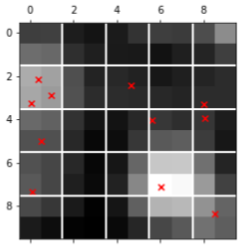
\includegraphics[width = 0.32\textwidth]{figures/vi_figures/example_tiled_less_whitespace.png}
%     \caption{Tiling a $10 \times 10$ pixel image into $2 \times 2$ tiles.}
%     \label{fig:ex_tiles}
% \end{wrapfigure}

\begin{figure}[tb]
    \centering
    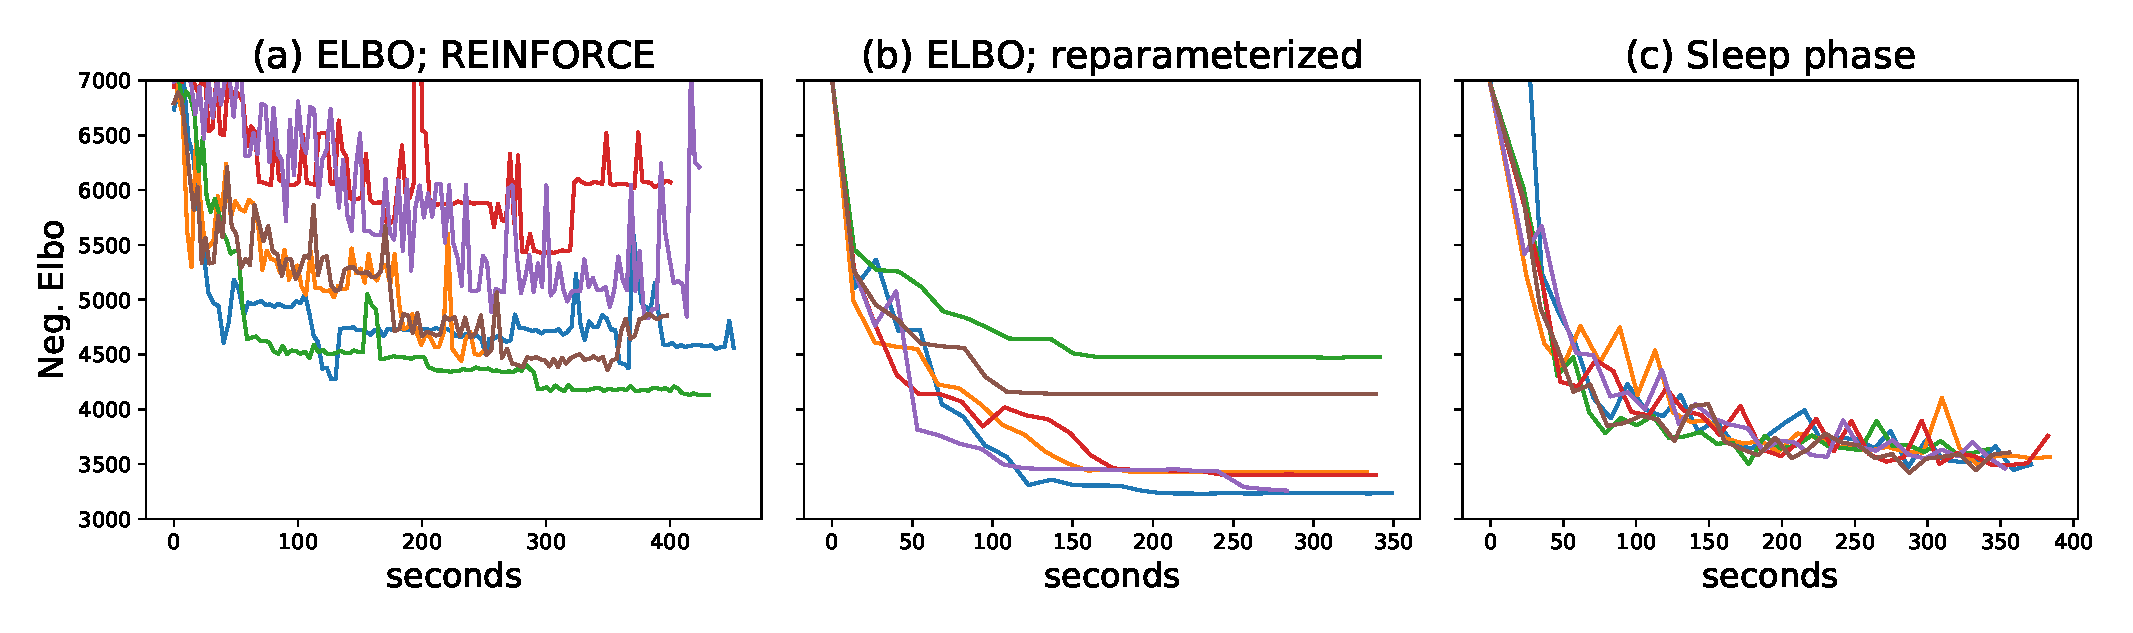
\includegraphics[width = 0.25\textwidth]{figures_vg/vi_figures/example_tiled_10.eps}
    \caption{Tiling a $20 \times 20$ pixel image into four $10 \times 10$ tiles.}
    \label{fig:ex_tiles}
\end{figure}

To make optimization tractable, the family $\mathcal{Q}$ is normally restricted to probability distributions
without conditional dependencies between some latent variables. In the most extreme case, known as mean-field variational inference, the variational distribution completely factorizes across all latent variables.

Our factorization has a spatial structure.
First, we partition the full $H \times W$-pixel image into disjoint $R \times R$-pixel tiles.
$R$ is chosen such that the probability of having three or more stars in one tile is small.
In this way, the cataloging problem decomposes to inferring only a few stars at a time (Section~\ref{sec:nn_architecture}).


Let $S = \sfrac{H}{R}$ and $T = \sfrac{W}{R}$ and assume without loss of generality that $H$ and $W$ are multiples of $R$.
For $s = 1, ..., S$ and $t = 1, ..., T$,
the tile $\tilde x_{st}$ is composed of the pixels
\begin{align}
    \tilde x_{st} = \{x_{hw} : Rs \leq h < R(s+1) \text{ and } Rt \leq w < R(t+1)\}.
    \label{eq:tiles}
\end{align}
Figure~\ref{fig:ex_tiles} gives an example with $R = 2$.

Let $\tilde N^{(s, t)}$ be the number of stars in tile $(s,t)$.
Because $\tilde N^{(s, t)}$ is random,
the cardinality of the set of locations and fluxes in each tile
is also random.
To handle the trans-dimensional parameter space,
we consider {\itshape triangular arrays} of latent variables
for each tile:
\begin{align}
    \tilde\ell^{(s, t)} &= (\tilde\ell_{N, i}^{(s, t)} : i = 1, ..., N; N = 1, 2, ...), \\
    \text{ and } \tilde f^{(s, t)} &= (\tilde f_{N, i}^{(s, t)} : i = 1, ..., N; N = 1, 2, ...),
\end{align}
where $\tilde\ell_{N, i}^{(s, t)}$ and $\tilde f_{N, i}^{(s, t)}$ are the elements of the triangular array corresponding to location and fluxes, respectively.
Tile locations $\tilde\ell_{N, i}^{(s, t)} \in [0, R]\times[0, R]$ give the location of stars within a tile. The fluxes $\tilde f_{N, i}^{(s, t)}$ are vectors in $\mathbb{R}^B_+$ (one flux for each band).

We refer to $(\tilde N^{(s, t)}, \tilde \ell^{(s, t)}, \tilde f^{(s, t)})_{s=1,t=1}^{S,T}$ as the {\itshape tile latent variables}. The distribution on tile latent variables factorize over image tiles:
\begin{align}
    \tilde q_\eta\big( \big(\tilde N^{(s, t)}, \tilde \ell^{(s, t)}, \tilde f^{(s, t)}\big)_{s=1, t = 1}^{S, T} \mid x\big)
    &=
    \prod_{s = 1}^S \prod_{t=1}^T
    \tilde q_\eta\big(\tilde N^{(s, t)}, \tilde \ell^{(s, t)}, \tilde f^{(s, t)} \mid x\big).
    \label{eq:factorize_patches}
\end{align}

We denote tile latent variables as $\tilde z$.
The ultimate latent variable of interest is $z = \{N, (\ell_i, f_{i,1}, ..., f_{i,B})_{i = 1}^N\}$, the catalog for the full image.
There is a mapping from $\tilde z$ to $z$.
First, the number of stars in the full catalog is given by the sum of the stars in each tile, $N = \sum_{s,t} \tilde N^{(s, t)}$.
Then, for every tile $(s,t)$, we index into the $\tilde N^{(s,t)}$-th row of the triangular array of tile latent variables $\tilde f^{(s,t)}$ and $\tilde \ell^{(s,t)}$.
The union of these fluxes and locations over all tiles form the full catalog (tile locations are shifted by the position of the tile in the full image to obtain locations in the full image).
See Figure~\ref{fig:tile_to_full_schm} for a schematic.


% \begin{align}
%     \{f_i\}_{i=1}^N = \Big\{\tilde f_{\tilde N^{(s, t)}, i}^{(s, t)} : i = 1, ..., \tilde N^{(s, t)}, s = 1, ..., S, t = 1, ..., T \Big\},
% \end{align}
% and the corresponding locations are
% \begin{align}
%     \{\ell_i\}_{i = 1}^N = \left\{\tilde \ell_{N^{(s, t)}, i}^{(s, t)} +
%     \begin{pmatrix}
%     Rs \\ Rt
%     \end{pmatrix}
%     : i = 1, ..., N^{(s, t)}, s = 1, ..., S, t = 1, ..., T\right\}.
% \end{align}
% The tile location is shifted by $(Rs, Rt)$ to obtain the location in the full image.

% Given this mapping from tile latent variables to the catalog of interest,
% \begin{align}
%  \big(\tilde N^{(s, t)}, \tilde \ell^{(s, t)}, \tilde f^{(s, t)}\big)_{s=1, t = 1}^{S, T}
% \mapsto
% \{N, (\ell_i, f_{i,1}, ..., f_{i,B})_{i = 1}^N\},
% \label{eq:patch_to_full_map}
% \end{align}
% a distribution on the tile latent variables induces a distribution on catalogs.

% Within each tile $(s,t)$, the distribution also fully factorizes:
% \begin{align}
%     \tilde q_\eta\big(\tilde N^{(s, t)}, \tilde \ell^{(s, t)}, \tilde f^{(s, t)} \mid x\big)
%     &=
%     \tilde q_\eta\big(\tilde N^{(s, t)} \mid x\big)
%     \prod_{n = 1}^\infty \prod_{i = 1}^n
%     \tilde q_\eta\big(\tilde \ell_{n,i}^{(s, t)} \mid x\big)
%     \tilde q_\eta\big(\tilde f_{n,i}^{(s, t)} \mid x\big).
%     \label{eq:factorize_within_patch}
% \end{align}

If $\tau$ is the mapping from $\tilde z$ to $z$,
then the variational distribution on catalogs $z$ is
\begin{align}
    q_\eta(z \mid x) := \tilde q_\eta(\tau^{-1}(z) \mid x),
    \label{eq:pull_back_of_q}
\end{align}
where $\tau^{-1}(z)$ is the pre-image of $z$ under $\tau$.
See Appendix~\ref{sec:eval_var_distr} for details on evaluating $q_\eta(z \mid x)$ for any given catalog $z$, which by \eqref{eq:pull_back_of_q} requires finding the pre-image $\tau^{-1}(z)$.


% for the figure
% {\color{blue} \tilde N^{(1,1)} = 2}

% \\

% \\

% \begin{pmatrix}
% (\tilde \ell, \tilde f)_{1, 1} & \\
% \color{blue} (\tilde \ell, \tilde f)_{2, 1} &
% \color{blue} (\tilde \ell, \tilde f)_{2, 2} &
% \end{pmatrix}^{(1,1)}

% \{{\color{Blue} N = 4},
% {\color{red} (\tilde \ell, \tilde f)^{(1,1)}_{2,1},
% (\tilde \ell, \tilde f)^{(1,1)}_{2,2}},
% {\color{DarkGreen} (\tilde \ell, \tilde f)^{(1,2)}_{1, 1}},
% {\color{Orange} (\tilde \ell, \tilde f)^{(2,1)}_{1, 1}}
% \}

\begin{figure}[tb]
    \centering
    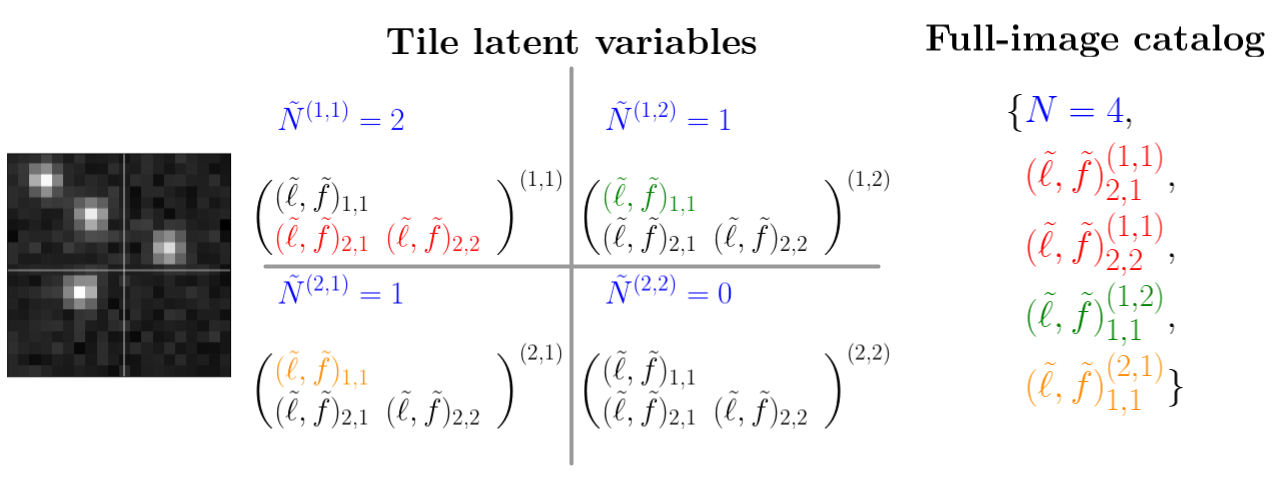
\includegraphics[width = 0.9\textwidth]{figures/vi_figures/tile_to_full_schematic.png}
    %\vspace{-0.6cm}
    \caption{An example image with four tiles and four stars illustrating the relationship between the tile latent variables and the full-image catalog.
    To construct the full-image catalog, we index into the appropriate row of the triangular array for each tile.}
    \label{fig:tile_to_full_schm}
\end{figure}


\subsection{Variational distributions on image tiles}
\label{sec:distr_on_tiles}
We describe the variational distribution for each tile,
$\tilde q_\eta\big(\tilde N^{(s, t)}, \tilde \ell^{(s, t)}, \tilde f^{(s, t)} \mid x\big)$.
The latent variables fully factorize within each tile.
Dropping the index
$(s,t)$ in this subsection,
\begin{align}
    \tilde N &\sim \text{Categorical}(
    \omega; 0, ..., N_{max});  \label{eq:var_distr_n}\\
	\tilde \ell_{j, i} / R &\sim \text{LogitNormal}(\mu_{\ell_{j, i}}, \text{diag}(\nu_{\ell_{j, i}}) )\label{eq:var_distr_loc}; \\
	\tilde f^b_{j, i} &\sim \text{LogNormal}(\mu_{f^b_{j, i}}, \sigma^2_{f^b_{j, i}}), \label{eq:var_distr_f}
\end{align}
independently for $i = 1, ..., j$; $j = 1, ..., N_{max}$.
Here $\omega$ is a $(\tilde N_{max} + 1)$-dimensional vector on the simplex. $\mu_{\ell_{j, i}}$ and $\nu_{\ell_{j, }}$ are two-dimensional vectors---the covariance on locations is diagonal.
Note that in the exact posterior, $\tilde N$ has support on the nonnegative integers, whereas in the variational distribution $\tilde N$ is truncated at some large $N_{max}$.


These distributions were taken to match the constraints of the latent variables: fluxes are positive and right skewed, suggesting a log-normal; locations are between zero and $R$, suggesting a scaled logit-normal.

\subsection{Neural network architecture}
\label{sec:nn_architecture}

In each tile, the distributional parameters in \eqref{eq:var_distr_n},
\eqref{eq:var_distr_loc}, and \eqref{eq:var_distr_f} are the output of a neural network.
The input to the neural network is an $R \times R$ tile, padded with surrounding pixels.
Padding enables the neural network to produce better predictions inside the tile.
For example, a bright source outside but in the vicinity of the tile affects the pixel values inside the tile.
Padding the tiles allows the neural network access to this information.
Thus, while the distribution on tile latent variables factorize over tiles, the neural network is able to use information from neighboring tiles in producing the distributional parameters.

The appropriate amount of padding will depend on the PSF width in the analyzed image.
To catalog the crowded starfield M2 (Section~\ref{sec:results_on_m2}),
we set $R = 2$ and padded the tile with a three-pixel-wide boundary.
In cataloging a DECam image, we use larger tiles with more padding because the width of the PSF is larger in these images. There, we set $R = 10$ and used a five-pixel-wide boundary.


% Let $\hat x^{(s,t)}$ denote the padded tile pixel intensities (which includes all $B$ bands) and $h_\eta$ be the neural network.
% which returns the collection of distributional parameters %in~\eqref{eq:var_distr_n}-\eqref{eq:var_distr_f} on tile $(s,t)$.
% \begin{align}
%     h_\eta(\hat x^{(s,t)}) = (\omega^{(s,t)}, \mu_\ell^{(s,t)}, \nu_{\ell}^{(s,t)}, \mu_f^{(s,t)}, \sigma^{(s,t)}_f).
%     \label{eq:nn_output}
% \end{align}
% The same neural network is evaluated for all tiles $(s,t)$.
In amortized inference, the variational parameters $\eta$ are neural network weights.
The architecture consists of a convolutional layer followed by several residual network layers, which themselves contain convolutions, before ending with several fully connected layers (Figure~\ref{fig:starnet_arch}).
This architecture has been successful on image classification challenges such as ImageNet~\citep{imagenet2015}.
We tuned the architecture using Optuna, an automatic hyper-parameter optimization package \citep{optuna_2019}. 
Our search included the number of convolution layers, 
the number of fully connected layers,
the number of channels in the convolution layers, and the size of the fully connected layers. 

An input to the network is a padded tile, which consists of $B$ color bands. 
We also append an additional ``band" to the input, which 
is a one-hot encoding with
ones for pixels inside the tile, and zeros outside. 
We do this because the network is only responsible for inferring sources inside each tile, and this additional band gives
the network access to a feature which encodes the tile interior. 

See Appendix~\ref{sec:supp_nn_architecture} for further details 
concerning the parameters of our neural network architecture. 
% our focus in this paper is the application of neural networks to provide a variational posterior for cataloging starfields, not the network architecture per se.


% Convolutional layers are useful for localizing stars, as they make the network invariant to shifts in stellar location. The convolutional kernel in the first layer is $3\times3$ pixels, roughly the full width at half maximum (FWHM) of the PSF.

\begin{figure}[!tb]
    \centering
    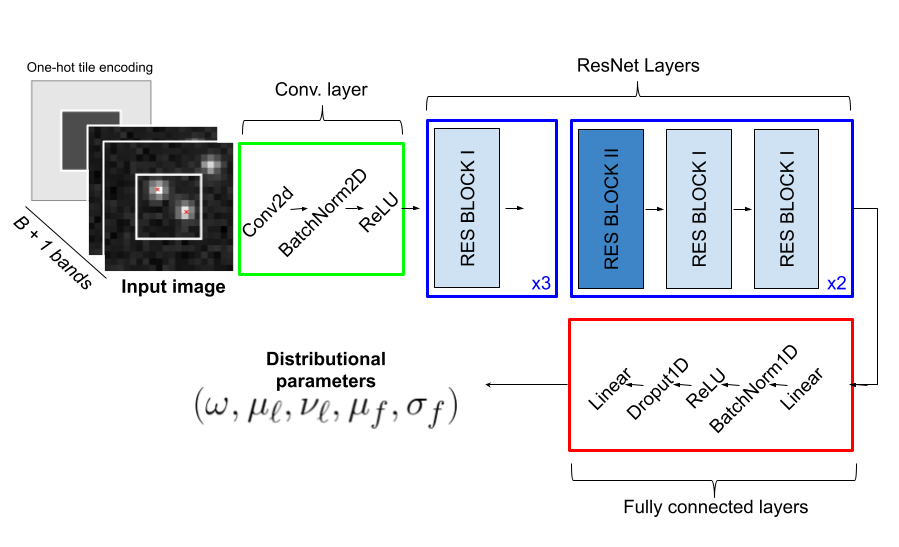
\includegraphics[width=\textwidth]{figures_vg/starnet_archetecture9.png}
%    \vspace{-1.cm}
    \caption{The neural network architecture. The DECam input is a two-band $20\times 20$ padded tile, 
    and the network returns distributional parameters corresponding to sources located in the $10\times 10$ tile outlined in white.
    In this example, there are two sources located in the $10\times10$ tile.
    The additional input band is a one-hot encoding with ones for pixels inside the tile, and zeros outside. 
    For further details concerning the residual network blocks (in blue), see 
    Appendix~\ref{sec:supp_nn_architecture}.
    }
    \label{fig:starnet_arch}
\end{figure}

% Note the output dimension of the neural network. For each tile $(s,t)$, the categorical parameter $\omega^{(s,t)}$
% lies on the simplex and has dimension $N_{max} + 1$.
% Furthermore, each index of the triangular array
% $i = 1, ..., \tilde N^{(s,t)}$, $\tilde N^{(s,t)} = 1, ..., N_{max}$
% describes a star. The star has a mean and variance for each location coordinate, and a mean and variance for its flux in each band.
% Thus, for each star $(\tilde N^{(s,t)}, i)$,
% the neural network outputs $2 \times (B + 2)$ parameters.
% In total, the neural network has output dimension $(N_{max} + 1) + (B + 2) \times (N_{max}^2 + N_{max})$.

% Recall that locations on the
% full image $\ell_{N, i}$ are parameterized to be in $[0, H] \times [0, W]$.
% On the tiles, locations $\ell^{(k)}_{N, i}$ are parameterized to be in
% $[0, s] \times [0, s]$.

Note that the output dimension of the neural network is quadratic in $N_{max}$: the outputs are parameters for a triangular array consisting of $\frac{1}{2}(N_{max}^2 + N_{max})$ sources.
Factorizing the variational distribution spatially keeps the output dimension manageable.
While the full image may contain many stars
(on the images that we catalog, the number of stars is on the order of thousands),
we set $N_{max} = 3$ for each tile.
Thus, the network is responsible for inferring only a few stars at once---a much easier task than inferring all stars simultaneously.

We emphasize that while the variational distribution factorizes over tiles, our method does not break the inference problem for the full image into isolated subproblems.
The likelihood of the full image does not factorize over tiles. Light from a star within a tile spills over into neighboring tiles, so the likelihood should not and does not decouple across image tiles.


\section{The wake-sleep algorithm}
\label{sec:wake_sleep}
\section{The expected forward Kullback-Leibler divergence}
\label{sec:wake_sleep}

% In mean-field variational inference, the ELBO~\eqref{eq:elbo} is often optimized by coordinate ascent in the parameters of the variational distribution.
% The coordinate ascent updates can be derived in closed form in the special case of exponential family models that are conditionally conjugate~\citep{Blei_2017_vi_review}.

Procedures such as black-box variational inference (BBVI)~\citep{ranganath2013black} and
automatic-differentiation variational inference (ADVI)~\citep{kucukelbir2016automatic}
optimize the ELBO  without the need for
deriving analytic expressions for the expectation over $q_\eta$.
% Examples of such ``automatic" procedures include
%and automatic-differentiation variational inference (ADVI)~\citep{kucukelbir2016automatic}.
These approaches employ stochastic gradient descent (SGD);
they sample latent variables from $q_\eta$ and produce an unbiased estimate for the gradient of the ELBO by taking advantage of modern automatic differentiation tools.
ADVI is closely related to the reparameterization trick \citep{SpallOptimization2003,kingma2013autoencoding, rezende2014stochastic}, which is often used to fit variational autoencoders and applies when the latent variables are continuous.

In our model, the number of stars $N$ is discrete.
The REINFORCE estimator~\citep{Williams1992reinforce} is one way to produce an unbiased stochastic gradient for both continuous and discrete latent variables.
However, REINFORCE gradients often suffer from high variance in practice, even with the introduction of control variates, resulting in slow convergence of stochastic optimization. We find this to be true in our empirical study (Section~\ref{sec:elbo_sleep_compare}).
% See Appendix~\ref{sec:reparam_details} for details concerning both the reparameterization and REINFORCE estimators.

The key difficulty in constructing stochastic gradients of the ELBO is that the
integrating distribution depends on the optimization parameter $\eta$.
We instead maximize a negated expectation of the ``forward" KL divergence:
\begin{align}
    \mathcal{L}_{fwd}(\eta) :=
    - \Expect_{x \sim p(x)}\Big[\KL(p(z \mid x) \| q_\eta(z \mid x))\Big]
    \label{eq:sleep_obj},
\end{align}
an objective that appears in the ``sleep phase" of the wake-sleep algorithm
\citep{Hinton1995wake_sleep, bornschein2014reweighted,le2020revisiting}
and was re-introduced by \cite{ambrogioni2019favi}, who called this approach ``Forward Amortized Variational Inference."

Section~\ref{sec:sleep_details} details a simple gradient estimator for~\eqref{eq:sleep_obj} that does not require reparameterization or REINFORCE.

There are two key differences between the expected forward KL objective~\eqref{eq:sleep_obj}
and the ELBO~\eqref{eq:elbo}.
First, recall that maximizing the ELBO is equivalent to minimizing
$\KL(q\|p)$; the KL in $\mathcal{L}_{fwd}$ transposes the arguments.
Second, the outer expectation over $p(x)$ in $\mathcal{L}_{fwd}$ gives a different meaning to the objective.
The ELBO objective seeks $\eta$ to minimize the $\KL$ between $q_\eta(z \mid x)$ and $p(z \mid x)$
for fixed, observed data $x$,
in this case the $H\times W$ image.
In contrast, minimizing $\mathcal{L}_{fwd}$ minimizes the $\KL$
on average over all possible data $x$,
as weighted by $p(x)$.
The target is no longer an approximate posterior for the observed data, but rather
an approximate posterior that is ``good on average" over all possible data under the model $p(x)$.

% Therefore, it is imperative that the model $p(x)$ approximates the true underlying data-generating mechanism well.
% Thus, the wake-sleep algorithm also incorporates a ``wake phase" to estimate model parameters.
% In our application, these model parameters include PSF parameters $\pi$ and background parameters $\beta$. Define
% $\phi:=(\pi, \beta)$, and denote the dependence of the generative model on $\phi$ using subscripts, $p_\phi$.
%
% To estimate model parameters, one would ideally optimize the marginal log-likelihood $\log p_\phi(x)$.
% However, since $\log p_\phi(x)$ is intractable, the wake-phase optimizes for $\phi$ using the ELBO~\eqref{eq:elbo}
% as a surrogate for the intractable log-likelihood.
% The ELBO is a lower bound of
% $\log p_\phi(x)$;
% it is equal to $\log p_\phi(x)$ when $q_\eta(z \mid x)$
% = $p_\phi(z \mid x)$.
%
% The {\itshape wake-sleep} algorithm alternates between the two objectives:
% \begin{align}
%     \text{{\bf Sleep phase: }} &
%     \eta_{t} = \argmax_{\eta} -\Expect_{x \sim p_\phi(x)}\Big[\KL(p_{\phi_{t-1}}(z \mid x) \| q_\eta(z \mid x))\Big]
%     \label{eq:sleep_phase_summary};
%     \\
%     \text{{\bf Wake phase: }} & \phi_{t} = \argmax_{\phi}\; \Expect_{q_{\eta_t}(z \mid x)}\Big[\log p_{\phi}(x, z) - \log q_{\eta_t}(z \mid x)\Big],
%     \label{eq:wake_phase_summary}
% \end{align}
% for iterations $t = 1, ..., T$.
%
% Stochastic gradients of the expectation in the wake-phase are simple to compute. Because the integrating distribution does not depend on the optimization parameter $\phi$ in the wake phase, unbiased stochastic gradients are simply computed as
% \begin{align}
%     \nabla_\phi \log p_\phi(x, z) \quad \text{ for } z\sim q_\eta.
%     \label{eq:mstep_grad}
% \end{align}
% Section~\ref{sec:sleep_details} shows that a similarly simple gradient estimator exists for the sleep objective.
%

% While the E-step~\eqref{eq:e_step} is not conducive to simple gradient estimators, we will see in Section~\ref{sec:sleep_details} that the sleep phase objective
% results in a similarly straightforward gradient estimator as in~\eqref{eq:mstep_grad}.
% In Section~\ref{sec:estep_sleep_compare},
% we compare optimizing the E-step with optimizing the sleep phase. In our application of localizing stars,
% the ELBO objective in the E-step suffers from poor local optima where the variational distribution is far from the true posterior in KL divergence; the sleep phase objective appears to better avoid these local optima.

% \subsection{Variational EM}
The wake-sleep algorithm is closely related to variational EM~\cite{Jordan_intro_vi, neal2000varem, Beal2002varem}, 
which alternates between an {\itshape expectation} step (E-step) and a {\itshape maximization} step (M-step): 
\begin{align}
    \text{{\bf E-step: }} & 
    \eta_{t} = \argmax_{\eta}\; \Expect_{q_\eta(z | x)}\Big[\log p_{\phi_{t-1}}(x, z) - \log q_\eta(z | x)\Big]; 
    \label{eq:e_step}
    \\
    \text{{\bf M-step: }} & \phi_{t} = \argmax_{\phi}\; \Expect_{q_{\eta_t}(z | x)}\Big[\log p_{\phi}(x, z) - \log q_{\eta_t}(z | x)\Big],
    \label{eq:m_step}
\end{align}
for iterations $t = 1, ..., T$. 

Variational EM can be viewed as block coordinate ascent on the ELBO objective, with the E-step optimizing variational parameters $\eta$ and the M-step optimizing the model parameters $\phi$. 

The wake phase of the wake-sleep algorithm is equivalent to the M-step of variational EM. 
As discussed above, the optimization of variational parameters $\eta$ using the ELBO objective is not conducive to using simple stochastic gradient estimators.
Thus, the sleep phase replaces the ELBO objective of the E-step with the expected reverse KL in~\eqref{eq:sleep_obj}.
\subsection{Decomposing the Expected Forward KL}
\label{sec:sleep_details}
In this subsection, we decompose the expected forward KL objective $\mathcal{L}_{fwd}$ 
to obtain an unbiased stochastic gradient for stochastic gradient descent. 

First, observe that optimizing $\mathcal{L}_{fwd}$ does not require computing the intractable term $p(x)$:
\begin{align}
\argmax_\eta\; \mathcal{L}_{fwd}(\eta)
    & = \argmin_{\eta} \; \mathbb{E}_{x \sim p(x)}\Big[ \mathrm{KL}(p(z \mid x) \| q_\eta(z \mid x)\Big] \\
  &=\argmin_{\eta} \; \mathbb E_{p(x)}\Big[\mathbb E_{p(z \mid x)}\Big(\log p(z \mid x) - \log q_\eta(z \mid x) \Big)\Big]\\
%&=\argmin_{\eta} \; \mathbb E_{p(x)}\Big[\mathbb E_{p(z \mid x)}\Big( - \log q_\eta(z \mid x) \Big)\Big]\\
&=\argmin_{\eta} \; \mathbb E_{p(x, z)}\Big[- \log q_\eta(z \mid x) \Big]\label{eq:sleep_loss_simple}.
\end{align}
Notice the integrating distribution $p(x,z)$ does not depend on the optimization parameter $\eta$.
% In the ELBO, the integrating distribution is $q_\eta$, resulting in the need for reparameterization or other adjustments to compute stochastic gradients.
Thus, unbiased stochastic gradients can be obtained as
\begin{align}
    g = -\nabla_\eta \log q_\eta(z \mid x) \quad \text{ for } (x, z)\sim p(x, z).
\end{align}

In other words, at each iteration of SGD, we simulate complete data $(x,z)$ from the generative model and evaluate the loss $-\log q_\eta(z \mid x)$.
Here, ``complete data" refers to the image along with its catalog.
This loss encourages the neural network to map an image $x$ to a distribution $q_{\eta}(\cdot \mid x)$ that places large density on the image's catalog $z$.

We decompose the loss $-\log q_\eta(z \mid x)$ further.
Recall that $q_\eta$ fully factorizes over tile latent variables, and thus $-\log q_\eta(z \mid x)$ is a summation over all tile latent variables.
To evaluate $-\log q_\eta(z \mid x)$ for some $(x,z)\sim p$, first convert $z$ to its tile parameterization $(\tilde N^{(s,t)}, \tilde \ell^{(s,t)}, \tilde f^{(s,t)})_{s=1,t=1}^{(S,T)}$, as detailed in Appendix~\ref{sec:eval_var_distr}.
For each tile $(s,t)$, the variational distribution on the number of stars $\tilde N^{(s,t)}$ is categorical with probability vector $\omega^{(s,t)}\in\Delta^{N_{max}}$ (recall Section~\ref{sec:distr_on_tiles}).
The loss function for the number of stars becomes
\begin{align}
    - \log q_\eta(\tilde N^{(s,t)} \mid x) = -\sum_{n = 0}^{\tilde N_{max}} 1\{\tilde N^{(s,t)} = n\} \log \omega^{(s,t)}_n.
    \label{eq:cross_entropy_loss}
\end{align}
The vector $\omega^{(s,t)}$ is the output of the neural network, and \eqref{eq:cross_entropy_loss} is the usual cross-entropy loss for a multi-class classification problem.

Next, recall that in the variational distribution location coordinates are logit-normal and fluxes are log-normal.
Let $y$ generically denote either the logit-location or log-flux for a star in the sampled catalog $z$; let $(\hat\mu, \hat\sigma^2)$ be the Gaussian mean and variance returned by the neural network. Then the loss for these latent variables is,
\begin{align}
    -\log q_\eta(y \mid x) =
        \frac{1}{2\hat\sigma^2}(y - \hat\mu)^2
         + \frac{1}{2}\log(2\pi\hat\sigma^2).
         \label{eq:gaussian_sleep_loss}
\end{align}
The first term encourages network predictions $\hat\mu$ to be close to the sampled latent variable $y$, while $\hat\sigma^2$ encodes the uncertainty of the network: the second term encourages small uncertainties, but is
balanced by the scaling of the error $(y - \hat\mu)^2$ in the first term.

% By our discussion in Section~\ref{sec:factorization},
% only the $N = N^{(s,t)}$-th row of the triangular
% array of latent variables $\tilde \ell^{(s,t)}$ and $\tilde f^{(s,t)}$ needs to be evaluated. Therefore, the losses in the last two terms of~\eqref{eq:sleep_loss_decomp} are of the form
% \begin{align}
%     -\log q_\eta(y \mid x) = -\sum_{i = 1}^{\tilde N^{(s,t)}} \log q_\eta(y_{\tilde N^{(s,t)},i} \mid x).
% \end{align}

% To interpret~\eqref{eq:gaussian_sleep_loss}, observe that
% $y_{n,i}$ is the true (simulated) latent variable in the catalog and
% $\mu_{n,i}$ is the predicted value for that latent variable from the neural network.
% $\sigma_{n,i}$ is also outputted by the neural network, representing uncertainty -- the second term encourages small uncertainties, but this is
% balanced by the scaling of the error $(y_{n,i} - \mu_{n,i})^2$ in the first term.

The losses in~\eqref{eq:cross_entropy_loss} and~\eqref{eq:gaussian_sleep_loss} show that the
expected forward KL objective results in a supervised learning problem on complete data
sampled from our generative model:
the objective function for the number of stars is the usual cross-entropy loss for classification,
while the objective function for log-fluxes and logit-locations are $L_2$ losses in the mean parameters.


% In Section~\ref{sec:estep_sleep_compare}, we will see the benefits of using complete data and optimizing $q_\eta$ using the losses~\eqref{eq:cross_entropy_loss} and \eqref{eq:gaussian_sleep_loss}  rather than the traditional ELBO.

% \subsubsection{Reverse versus forward KL}
% \label{sec:kl_q_p}
% TODO: something about forward KL overestimates uncertainties, see Figure~\ref{fig:kl_q_p_schematic}.

% \begin{figure}[!ht]
%     \centering
%     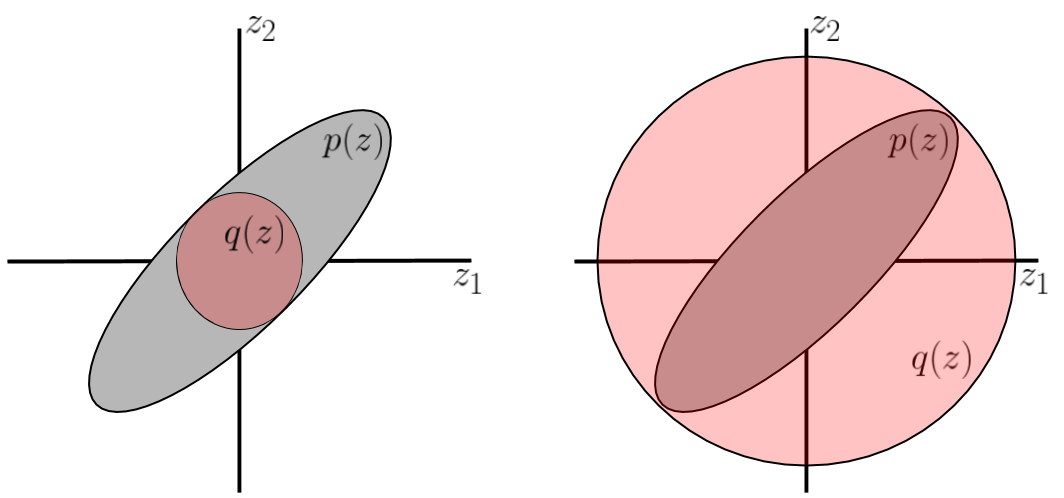
\includegraphics[width = 0.5\textwidth]{figures/kl_q_p_schematic.png}
%     \caption{A toy example where the target distribution $p$ is a bivariate Gaussian on
%     $z = (z_1, z_2)$ with positively correlated components.
%     $q$ is a mean-field variational approximation. Left, the optimal $q$ found
%     optimizing $\KL(q\|p)$; right, the optimal $q$ found optimizing $\KL(p\|q)$. }
%     \jeff{Are the contour lines for $p$ and $q$ the same (e.g., the contour that contains 50\% of the mass)? If so, is it true that these contours touch at exactly two point (rather than 0 or 4)? We should be correct on this detail if we're going to the trouble of showing a plot, even if we're just trying to get intuition.}
%     \label{fig:kl_q_p_schematic}
% \end{figure}

% NO LONGER NEEDED
% \section{Related work}
% \label{sec:related_work}
% % \subsection{Connection with variational EM}
% Wake sleep was originally proposed by~\cite{Hinton1995wake_sleep}, and revisited in~\cite{bornschein2014reweighted, le2018revisiting}. \cite{le2018revisiting} proposed wake-sleep as a viable alternative to the reparameterization trick when training discrete-distribution latent variable models. 

% We also note the connection between wake-sleep and variational EM~\cite{Jordan_intro_vi, neal2000varem, Beal2002varem}. For iterations $t = 1, ..., T$, variational EM alternates between two objectives: 
% \begin{align}
%     \text{{\bf E-step: }} & 
%     \eta_{t} = \argmin_\eta \; \mathrm{KL}\big (q_{\eta    }(N, \ell, f |X) \| P_{\phi_{t - 1}}(N, \ell, f | X)\big)
%     \label{eq:e_step}
%     \\
%     \text{{\bf M-step: }} & \phi_{t} = \argmin_{\phi} \; \mathrm{KL}\big (q_{\eta_t}(N, \ell, f |X) \| P_{\phi}(N, \ell, f | X)\big)
%     \label{eq:m_step}
% \end{align}
% The M-step in variational EM and the wake phase in wake-sleep are the same (compare equations~\eqref{eq:wake_kl} and \eqref{eq:m_step}). 
% Variational EM can be viewed as coordinate descent on the KL, with each step alternating between updating $\eta$ and $\phi$. The overall objective is 
% \begin{align}
% (\eta^*, \phi^*) = \argmin_{\phi, \eta} \; \mathrm{KL}\big (q_{\eta}(N, \ell, f |X) \| P_{\phi}(N, \ell, f | X)\big)\label{eq:em_obj}
% \end{align}

% The sleep phase is analogous to the E-step (compare equation~\eqref{eq:sleep_kl} and \eqref{eq:e_step}). 
% The sleep phase objective reverses the arguments of the KL in the E-step so it becomes more amenable to stochastic gradient methods. However, wake-sleep is no longer optimizing a single objective as in equation~\ref{eq:em_obj}. 

% \subsection{Cataloging of stellar fields}
% TODO

SDSS has a default cataloger, PHOTO~\cite{lupton2001sdss}. It timed out on the crowded starfield that we examine, M2. 

DAOPHOT~\cite{stetson2987daophot} is an algorithmic routine designed for crowded starfields. To detect stars, the observed image is convolved with a Gaussian kernel. The convolved image is scanned for peaks above a given threshold, which are then labeled as stars. \cite{An_2008_m2} applied DAOPHOT to catalog M2, and we refer to this as the DAOPHOT catalog in our comparisons. 

\cite{Brewer_2013, Portillo_2017, Feder_2019} employed probabilistic cataloging, and inference was using MCMC. In the most recent work \cite{Feder_2019}, a runtime of 30min was reported to catalog a $100 \times 100$ subimage of M2. In the sequel, we will compare the catalog produced from their MCMC procedure against the catalog produced by our variational posterior. We will show that our method is several orders of magnitude faster at inference time. 

Our generative model is most similar to \cite{Portillo_2017, Feder_2019}, except they used an exponential prior on the number of stars instead of Poisson. 
In \cite{Brewer_2013}, a broken power-law prior was used for the flux, and further hyper-priors are placed on the parameters of the broken power-law. The parameters of the broken power-law are treated as latent variables. In our case, this would be analogous to placing a hyper-prior on $\alpha$ from equation~\eqref{eq:flux_prior}. 
Alternatively, though not explored in this work, we can treat our prior parameter as a model parameter and optimize them in the wake phase. The same principle applies to the Poisson prior parameter, $\mu$. 

Finally, \cite{Portillo_2017, Feder_2019} use the default SDSS estimates. As will be shown in the sequel, the default SDSS estimates for the PSF and background can be improved for a better model fit. $\cite{Brewer_2013}$ treats the PSF parameters as latent variables in their MCMC chain. In contrast, 
our we estimate model parameters in the wake phase. 

\section{Empirical comparison of ELBO optimization and sleep optimization}

% Section~\ref{sec:estep_sleep_compare} motivates the wake-sleep approach by comparing variational posteriors obtained by optimizing the ELBO against those obtained by optimizing the sleep objective.
% Then, StarNet is tested on blended simulated stars in Section~\ref{sec:deblending_test}.
% Finally, in Section~\ref{sec:results_on_m2}, StarNet is employed to catalog the SDSS image of the M2 globular cluster. The StarNet catalog is compared with existing cataloging methods.

\label{sec:elbo_sleep_compare}

A simple example demonstrates that there exist shallow local optima in the ELBO
where the fitted approximate posterior is far in KL divergence from the exact posterior.
These local optima result in unreliable catalogs.
The expected forward KL, by taking advantage of complete data, appears to have a more favorable optimization landscape.
The simulated $20\times20$ single-band image $x_{test}$ is shown in Figure~\ref{fig:optim_path}(d).

We compare three approaches to deblending. The first two approaches directly optimize the ELBO,
\begin{align}
\mathcal{L}_{elbo}(\eta; x) = \Expect_{q_{\eta}(z \mid x)}\Big[\log p(x, z) - \log q_{\eta}(z \mid x)\Big],
\label{eq:elbo_on_test}
\end{align}
evaluated at $x = x_{test}$. 
The third approach minimizes the expected forward KL~\eqref{eq:sleep_obj}.
In each case, $q_\eta$ is the inference network from Section~\ref{sec:nn_architecture}.
The input to the network is a $10\times 10$ tile with no padding.

Note that the expected forward KL does not depend on $x_{test}$.
Optimizing $\mathcal{L}_{fwd}$ only requires sampling catalogs from the prior
and simulating images conditional on each catalog.
The prior on the number of stars was set to Poisson with mean $\mu = 4$.

Figure~\ref{fig:optim_path}~(top row) charts the test ELBO~\eqref{eq:elbo_on_test}
as optimization proceeds in our three approaches.
The first approach optimizes the ELBO with SGD and a REINFORCE plus control-variate gradient estimator~\citep{ranganath2013black}.
The path of the ELBO objective in this first approach is irregular, likely due to the high variance of the REINFORCE gradient estimator, 
and the optimization does not appear to converge (Figure~\ref{fig:optim_path}a).
For a lower-variance gradient estimator, the second approach employed the reparameterized gradient. To employ this gradient estimator, we analytically integrated the ELBO with respect to the number of stars $N$ to remove the discrete random variable.
See Appendix~\ref{sec:reparam_details} for details about the gradient estimators.
Using reparameterized gradients instead of REINFORCE gradients enabled the optimization to converge to stationary points (Figure~\ref{fig:optim_path}b).
However, for two randomly initialized restarts,
the optimization found local optima where the negative ELBO is notably higher than other restarts.

These shallow local optima in the ELBO result in unreliable catalogs.
The bottom row of Figure~\ref{fig:optim_path} displays the estimated locations, defined as the mode of the fitted variational distribution.
Figure~\ref{fig:optim_path}(e) shows these locations after converging to a shallow local optimum.
Here, the upper left tile was correctly estimated to have two stars, but both estimated stars were incorrectly placed at the same location.
(One of the locations should be placed on the second star.)
To move one of the estimated locations to the second star, the optimization path must traverse a region where the log-likelihood is lower than the current configuration (Figure~\ref{fig:local_optima_cartoon}).
The displayed configuration is a local optimum where the gradient with respect to its locations is approximately zero.

One the other hand, using
the expected forward KL does not directly optimize the test ELBO.
However, the test ELBO increases nonetheless, because the variational posterior
better approximates the exact posterior as the optimization proceeds.
Optimizing $\mathcal{L}_{fwd}$ consistently converged to
a similar ELBO across all restarts and avoided shallow local optima (Figure~\ref{fig:optim_path}c).
The expected forward KL is quadratic in the logit-location estimate
$\mu_\ell$ (\ref{eq:gaussian_sleep_loss}),
and the gradient does not vanish.
By avoiding shallow local optima, the variational distribution fit with the forward KL
always placed its mode on the four true stars in our trials.
An example of successful detection by fitting with
$\mathcal{L}_{fwd}$ is shown in~Figure~\ref{fig:optim_path}(f).

\begin{figure}[!htb]
    \centering
    \begin{subfigure}[t]{0.9\textwidth}
    \centering
    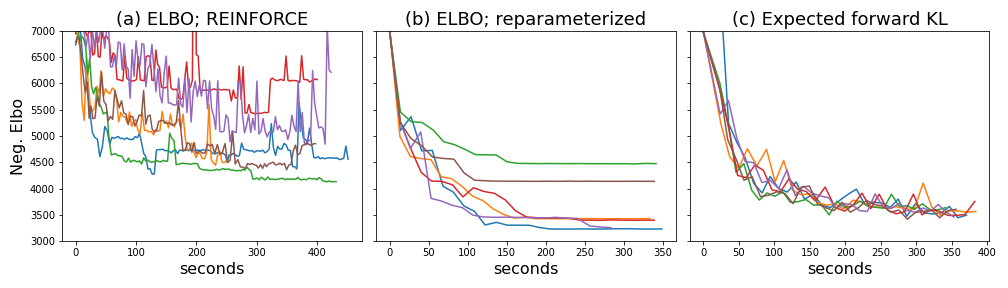
\includegraphics[width=\textwidth]{figures/elbo_vs_sleep/optim_path_compare.png}
    \end{subfigure}
    \begin{subfigure}[t]{\textwidth}
    \centering
    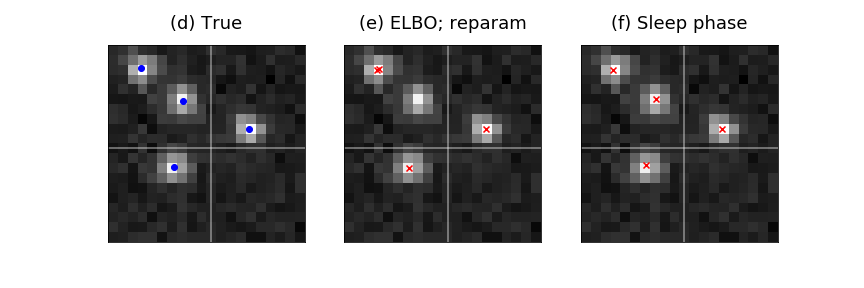
\includegraphics[width=0.9\textwidth]{figures/elbo_vs_sleep/optim_path_detect_compare.png}
    \end{subfigure}
    \vspace{-1.5cm}
    \caption{(Top row) The negative ELBO as the optimization progresses for six random restarts.
    (Bottom row) In red, modal locations from ELBO-optimized and $\mathcal{L}_{fwd}$-optimized variational posteriors, for one of the six restarts.
    In blue, the true locations. }
    \label{fig:optim_path}
\end{figure}

% Figure~\ref{fig:gradzero_cartoon} shows a schematic of the optimization landscape as a function of locations.
% Recall that locations are parameterized between 0 and 1, and the neural network returns a variational mean parameter $\mu_\ell$ for the logit-location.
% When $\mu_\ell$ is far from the correct location (in logit space), the gradient of the ELBO with respect to $\mu_\ell$ vanishes.
% To see this, observe that the PSF is nearly zero everywhere except for a few pixels around its center. Therefore, a small shift in estimated location $\mu_\ell$ does not significantly change the likelihood unless the estimated location is within a ``PSF radius" of the correct location.
% On the other hand, the sleep objective is quadratic in the logit-location estimate $\mu_\ell$ (see Equation~\ref{eq:gaussian_sleep_loss}).
% Thus, the further the estimated location is from the correct location (in logit space), the larger the gradient. The gradient does not vanish in the sleep objective.

\begin{figure}[!htb]
    \centering
    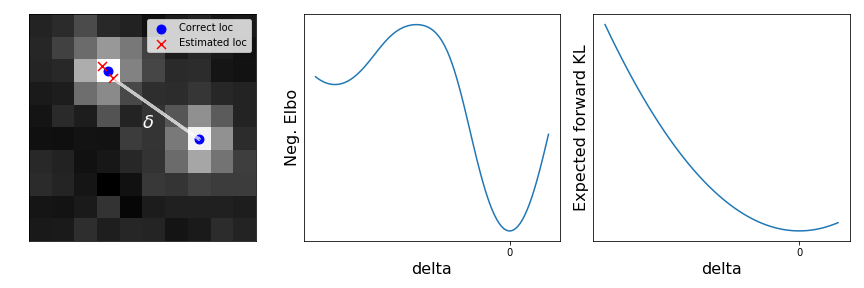
\includegraphics[width=0.9\textwidth]{figures/elbo_vs_sleep/local_minima_cartoon.png}
    \vspace{-0.5cm}
    \caption{An illustration of local optima in the ELBO objective.
    To move an estimated location to a correct location,
    the optimization path must traverse a region where the negative ELBO is larger than the current configuration.
    In contrast, when optimizing the expected forward KL with SGD, each iteration evaluates a
    quadratic loss between the true and estimated location,
    and the gradient does not vanish. }
    \label{fig:local_optima_cartoon}
\end{figure}

Finally, note that low-variance gradients of the ELBO for this simple example were constructed by analytically integrating out $N$, 
and this was only possible because the image consisted of only four tiles. 
For each tile, the variational distribution has support over only 0, 1, or 2 stars.
Since the variational distribution factorizes over the four tiles, integrating $N$ is a summation of $3^4 = 81$ terms.
On larger images with more tiles, analytically integrating $N$ would be computationally infeasible,
and the standard reparameterization trick would not apply as it does in this small illustrative example.

% On a larger images where $N$ is on the order of $\sim1000$ (e.g. on M2), analytically integrating out $N$ would be infeasible.

% Only then could the reparameterization trick be applied to the ELBO, as the remaining latent variables are continuous.

% In this example, the variational distribution has support over only 0, 1, or 2 stars for each tile.
% Since the variational distribution factorizes over the four tiles, integrating $N$ is a summation of $3^4 = 81$ terms.
% On larger images with more tiles, analytically integrating $N$ would be computationally infeasible,
% and the simple reparameterization trick would not apply as it does in this small illustrative example.

% Figure~\ref{fig:sim_data100x100} displays our results on a larger example: a simulated $100\times 100$ pixel image with fifty stars.
% The tiles again consisted of $10\times 10$ pixel regions.
% Optimizing the ELBO does not produce accurate location estimates and appears to be hindered by regions with little gradient information; optimizing the sleep objective produced much improved location estimates.


% \begin{figure}[!htb]
%     \centering
%     \begin{subfigure}[!t]{0.59\textwidth}
%     \centering
%     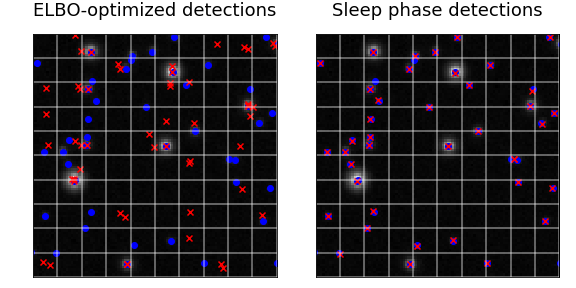
\includegraphics[width=\textwidth]{figures/elbo_vs_sleep/optim_path_detect_compare_100x100.png}
%     \end{subfigure}
%     \begin{subfigure}[!t]{0.4\textwidth}
%     \centering
%     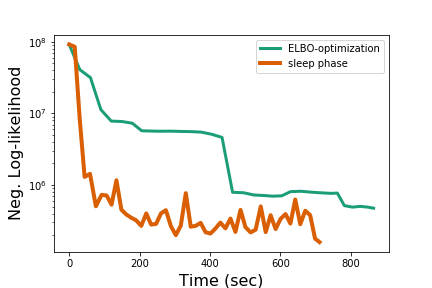
\includegraphics[width=\textwidth]{figures/elbo_vs_sleep/optim_path_compare_100x100.png}
%     \end{subfigure}
%     \caption{
%     (Left) Detections produced by ELBO optimization on a $100\times 100$ pixel test image.
%     Correct locations are blue and estimated locations are red.
%     (Middle) Detections produced by the sleep phase optimization.
%     (Right) The negative conditional log-likelihoood, $-\log p(x|\hat z)$, where $\hat z$ is the mode of the variational posterior and $x$ the
%     $100\times 100$ pixel test image. }
%     \label{fig:sim_data100x100}
% \end{figure}

% \subsection{A deblending test}
\label{sec:deblending_test}

We demonstrate the performance of StarNet on deblending two stars. Two stars were simulated in an $7\times 7$ image with two bands. 
The input to StarNet was the entire $7\times 7$ image; no tiling was used in this experiment. 
We fitted StarNet using the sleep phase, with prior described in Section~\ref{sec:gen_model}, except that the number of stars was uniform: with equal probability, there is either 0, 1, or 2 stars in the image. 

Figure~\ref{fig:deblending_fig} displays the probability that $N = 2$ under the fitted variational posterior, as the distance between two stars varies.
As expected, the probability of $N=2$ increases as the separation increases. 
In addition, the stars become easier to deblend as the flux increases (Figure~\ref{fig:deblending_fig}a).
In Figure~\ref{fig:deblending_fig}b, the flux of the first star was set at 4000nelec, and the flux of the second star was varied. 
As the difference in flux between the two stars increases, the stars become harder to deblend. 
Finally, in Figure~\ref{fig:deblending_fig}c, the flux of the first star was set at 4000nelec in both bands. The second star had flux 4000nelec in the first band, and its flux in the second was varied. 
This demonstrates the benefits of multiband deblending: color, 
the relative fluxes in neighboring bands, aids in differentiating stars. 

\begin{figure}[!h]
    \centering
    \begin{subfigure}{0.95\textwidth}
        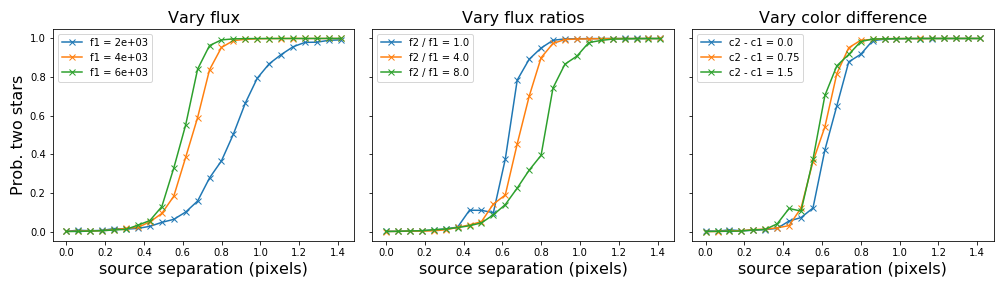
\includegraphics[width=\textwidth]{figures/deblending_test.png}
    \end{subfigure}
      \begin{subfigure}{0.95\textwidth}
        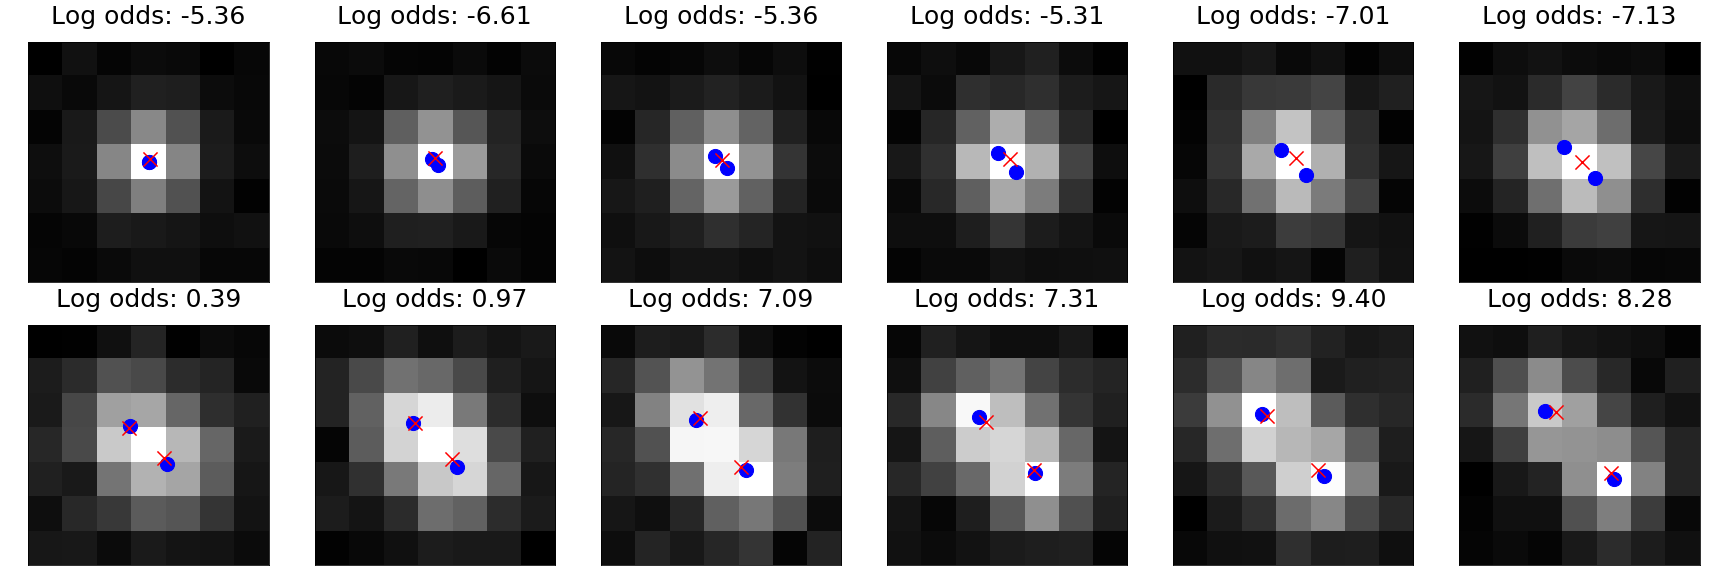
\includegraphics[width=\textwidth]{figures/deblending_ex.png}
    \end{subfigure}
    \caption{(Top row) The probability under $q$ that the image region contains two stars as source separation increases.
    (Bottom) An example of StarNet detections as source separation increases. Red are estimated locations, defined by the the mode of the variational distribution; blue are true locations. Log odds are probability of two stars over probability of one star. Here, both stars have a flux of 4000nelec.}
    \label{fig:deblending_fig}
\end{figure}


\section{Results on the M2 globular cluster}
First, we validate StarNet using an SDSS image of the Messier 2 (M2) globular cluster,
a crowded starfield found in field 136 of camera column 2 in run 2583.
M2 was also imaged in the ACS Globular Cluster Survey~\citep{Sarajedini_2007}
using the Hubble Space telescope (HST),
which has greater resolution than the Sloan telescope.
The resolution of the HST wide-field channel is 0.05 arcseconds per pixel versus
0.4 arcseconds per pixel in SDSS \citep{hubble_about, sdss_about}.
For this image, whe catalog from this Hubble survey (henceforth the ``HST catalog")
serves as ground truth for validating our results.

Then, we run StarNet on a frame from the DECam survey,
and demonstrate the ability of StarNet to scale to large astronomical surveys.

\subsection{Results on the M2 globular cluster}
\label{sec:results_on_m2}

We first focus on the $100 \times 100$ pixel subimage of M2 that
\cite{Portillo_2017} and \cite{Feder_2019} analyzed with PCAT.
This subimage is located approximately two arcseconds from the heavily saturated core of the cluster;
even in this subimage, the HST catalog contains over 1000 stars with F606W-band magnitudes less than 22.
We include two bands in our model, the SDSS $r$-band and $i$-band.
The SDSS $r$-band and the Hubble F606W band are centered at roughly the same wavelength,
but the wavelength range of the Hubble F606W band is slightly broader.

The cataloging accuracy of StarNet is compared with PCAT and DAOPHOT~\citep{stetson2987daophot}.
DAOPHOT is an algorithmic routine for detecting stars in crowded starfields which does not use a generative model.
This software convolves the observed image with a Gaussian kernel and scans for peaks above a given threshold.
The DAOPHOT catalog of M2 was reported in \cite{An_2008_m2}.


% Both DAOPHOT and the Hubble survey produce a single catalog -- that is, a set of estimated stellar locations and fluxes -- with
% error bars nominally representing marginal uncertainties.
% In the context of probabilistic cataloging (StarNet and PCAT), the posterior
% defines a distribution over catalogs.
% Each sample from the (approximate) posterior returns a catalog, and each
% sampled catalog may have different cardinally.

To evaluate the three methods, the HST catalog was used as ground truth.
We filtered the HST catalog to stars with magnitudes smaller than 22.5 in the Hubble F606W band,
because stars with lower apparent brightness cannot be detected in SDSS images.


Estimated catalogs are evaluated on three metrics: the true positive rate (TPR),
the positive predicted value (PPV), and the F1 score.
The TPR is the proportion of stars in the HST catalog matched with a star in the estimated catalog;
the PPV is the proportion of stars in the estimated catalog matched with a star in the HST catalog.
The F1 score summarizes the two metrics as the harmonic mean of the PPV and the TPR.

Like \cite{Portillo_2017} and \cite{Feder_2019}, a ``match" between an estimated star
and an HST star is defined as follows: (1) the estimated location and the HST location are within 0.5 SDSS pixels,
and (2) the estimated SDSS $r$-band flux and the HST F606W band flux are within half a magnitude.
% The slack in magnitude accounts for the fact that the wavelength range of the HST F606W band is slightly broader than the SDSS $r$-band (though they are centered at roughly the same wavelength).

In probabilistic cataloging (PCAT and StarNet), the posterior defines a distribution over catalogs.
For StarNet, the TPR, PPV, and F1 score were computed for the catalog corresponding to the mode of the variational distribution (henceforth, the StarNet catalog).
For PCAT, 300 catalogs were sampled using MCMC; the metrics were computed for each sampled catalog and averaged.

\begin{figure}[tb]
    \centering
    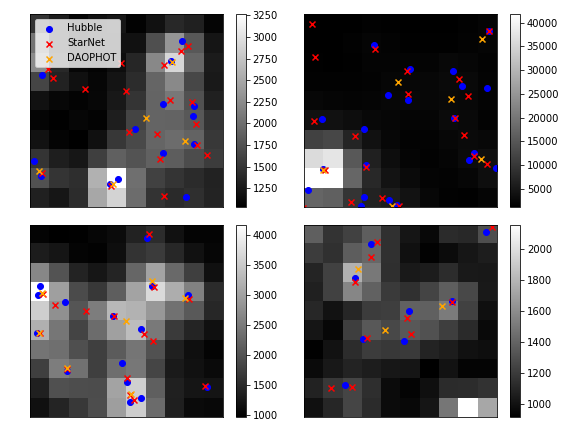
\includegraphics[width=0.49\textwidth]{figures/m2_results/example_subimages_starnet.png}
    \rulesep
    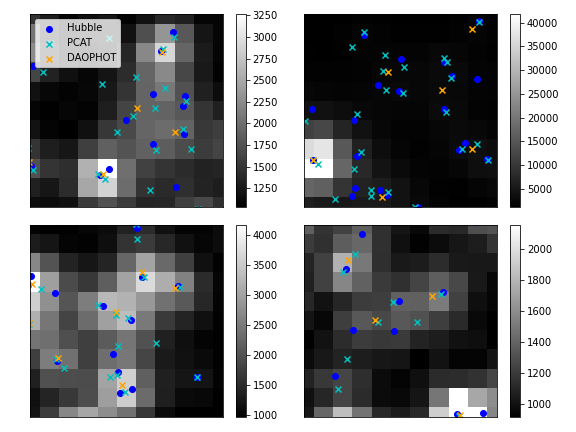
\includegraphics[width=0.49\textwidth]{figures/m2_results/example_subimages_pcat.png}
    % \vspace{-1cm}
    \caption{Estimated catalogs on four 10$\times$10 subimages from
    M2. Blue dots are stars from the HST catalog used as ground truth.
    Starnet, PCAT, and DAOPHOT estimated stars are shown as
    red, cyan, and orange crosses, respectively. }
    \label{fig:example_subimages}
\end{figure}

StarNet produced a catalog that outperforms DAOPHOT and PCAT in F1 score (Table~\ref{tab:summary_stats}).
Figure~\ref{fig:example_subimages} shows the StarNet catalog alongside PCAT, DAOPHOT, and HST catalogs.
DAOPHOT estimated less than half the number of stars when compared to the other methods.
It therefore had a large PPV but a small TPR.
The StarNet catalog had about the same TPR as PCAT while being ten points higher in PPV.

Table~\ref{tab:summary_stats} also prints the number of stars inferred by each method.
For probabilistic methods (StarNet and PCAT),
 we display the mean number of stars under the approximate posterior, along with the 5-th and 95-th quantiles.
There are 1114 stars in the HST catalog.
Neither PCAT nor StarNet captured the true number of stars in their 90\% credible interval,
but the StarNet credible intervals were three times wider than the PCAT intervals.
The small PCAT credible intervals may be indicative of an MCMC sampler that failed to mix well.

% \begin{table}[!tb]
% \centering
% \caption{Performance metrics on M2.
% For probabilistic methods (StarNet and PCAT)
% the ``\#stars" column refers to the mean number of stars under the (approximate) posterior, while the right-most column displays the 5-th and 95-th percentiles under the posterior. }
% \label{tab:summary_stats}
% \begin{tabular}{l|ccc|cc}
% \toprule
%      Method &   TPR &   PPV &  F1 score &  \#stars & (q-5\%, q-95\%)\\
% \midrule
%     DAOPHOT &  0.20 &  0.63 &      0.30 &     295 & -- \\
%        PCAT &  0.56 &  0.40 &      0.47 &    1672 & (1664, 1680)\\
%  Sleep-only &  0.51 &  0.47 &      0.49 &    1292 & (1260, 1324)\\
%  Wake-sleep &  0.51 &  0.60 &      0.55 &     1014 & (987, 1041)\\
%      %Hubble &  1.00 &  1.00 &      1.00 &     1114 & -- %\\
% \bottomrule
% \end{tabular}
% \end{table}

\begin{table}[!tb]
\centering
\caption{Performance metrics on M2.
For probabilistic methods (StarNet and PCAT)
the ``\#stars" columns provide the mean along with the 5th and 95th percentiles
for the number of stars under the (approximate) posterior,
The number of stars in the Hubble catalog is 1114. }
\label{tab:summary_stats}
\begin{tabular}{l|ccc|cc}
\toprule
& & & & \multicolumn{2}{c}{\#Stars} \\
     Method &   TPR &   PPV &  F1 score &  mean & (q-5\%, q-95\%)\\
\midrule
    DAOPHOT &  0.20 &  0.65 &      0.31 &     357 & -- \\
       PCAT &  0.55 &  0.37 &      0.44 &    1672 & (1664, 1680)\\
 StarNet (our) &  0.53 &  0.48 &      \textbf{0.50} &    1462 & (1430, 1497)\\
\bottomrule
\end{tabular}
\end{table}


The improvement of StarNet over PCAT in PPV was most pronounced for dim stars (Figure~\ref{fig:summary_stats}).
The TPR for StarNet was uniformly better than DAOPHOT across almost all magnitudes.
Of all methods, StarNet best approximated the HST flux distribution (Figure~\ref{fig:luminosity_fun_m2}).
% PCAT overestimated the number of dim stars with magnitudes greater than 21.
% In contrast, DAOPHOT failed to find stars with magnitudes greater than $21$.

% (Figures~\ref{fig:m2_flux_estimation} and \ref{fig:luminosity_fun_m2}).

\begin{figure}[tb]
    \centering
    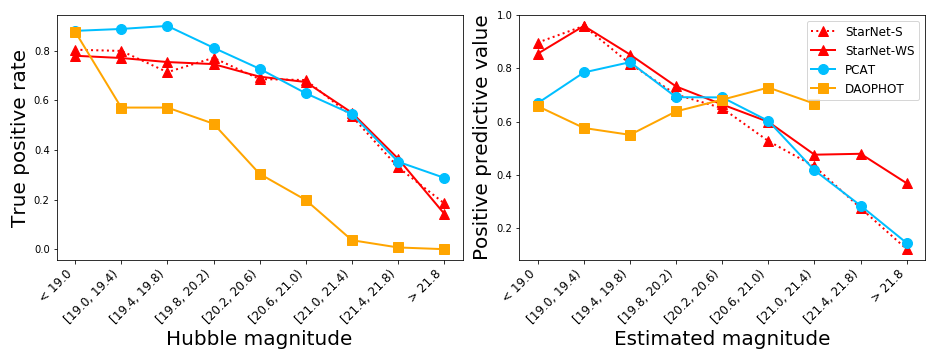
\includegraphics[width=0.99\textwidth]{figures/m2_results/summary_statistics_m2.png}
    \vspace{-0.4cm}
    \caption{True positive rate (left) and positive predicted value (right) of various cataloging
    procedures on M2, plotted against $r$-band magnitude.
    Smaller magnitudes correspond to brighter stars.
    }
    \label{fig:summary_stats}
\end{figure}

% \begin{figure}[tb]
%     \centering
%     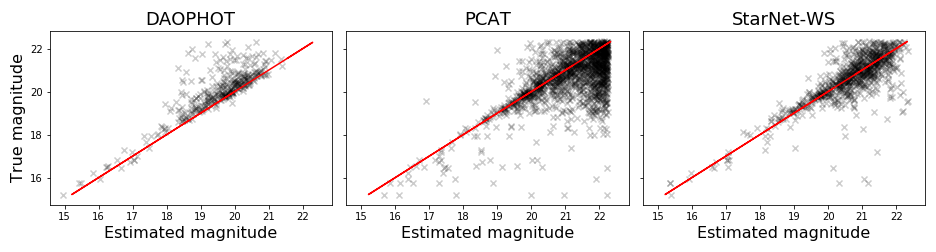
\includegraphics[width=0.99\textwidth]{figures/m2_results/m2_flux_estimation.png}
%     \caption{True versus estimated magnitudes on the $r$-band of M2.
%     Every estimated star was matched with the nearest Hubble star in L2 distance between locations.
%     Red line is the identity, $y=x$. }
%     \label{fig:m2_flux_estimation}
% \end{figure}

\begin{figure}[tb]
    \centering
    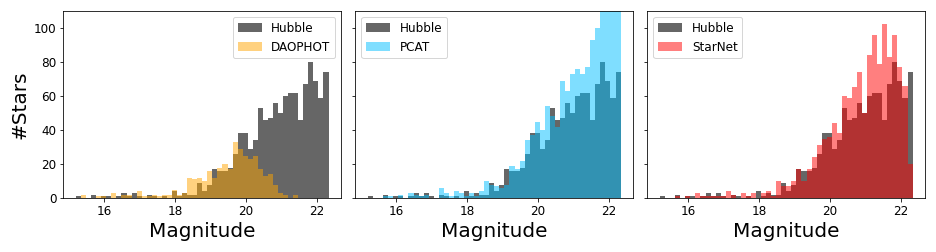
\includegraphics[width=0.99\textwidth]{figures/m2_results/luminosity_fun.png}
    \vspace{-0.4cm}
    \caption{Flux distributions for the $r$-band observations of M2.
    The flux distribution of the HST catalog in grey.
    Estimated distributions by DAOPHOT, PCAT, and StarNet-WS catalogs overlaid.
    For PCAT, the flux distribution is from a single catalog sample. }
    \label{fig:luminosity_fun_m2}
\end{figure}


% \begin{figure}[tb]
%     \centering
%     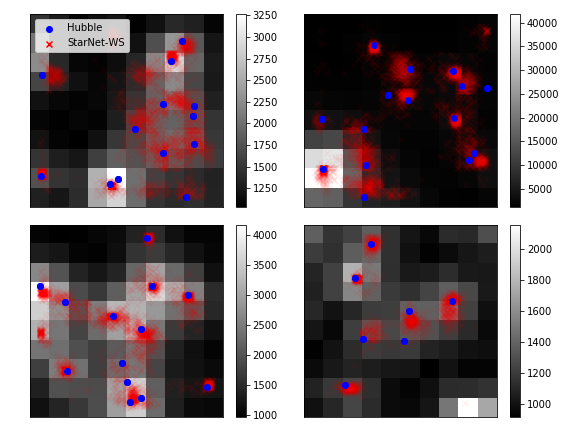
\includegraphics[width=0.49\textwidth]{figures/m2_results/example_subimages_samples_ws.png}
%     \rulesep
%     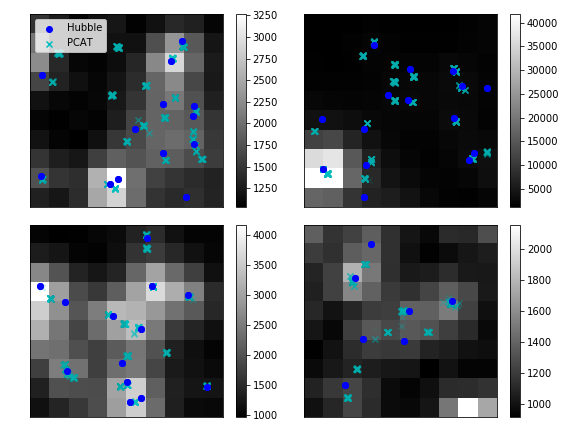
\includegraphics[width=0.49\textwidth]{figures/m2_results/example_subimages_samples_pcat.png}
%     \caption{Four 10$\times$10 subimages from
%     M2. Blue dots are stars from the HST catalog used as ground truth. (Left) Posterior samples from StarNet-WS and (right) posterior samples from the MCMC chain of PCAT. }
%     \label{fig:example_subimages_sampled}
% \end{figure}

% StarNet-WS returns a well-defined distribution over the set of all catalogs
% and is thus able to capture uncertainties in catalog construction.
% Samples from the StarNet-WS variational distribution are compared with samples from PCAT in Figure~\ref{fig:example_subimages_sampled}.
To examine the uncertainty calibration of StarNet, we evaluated the approximate posterior
conditional on the true number of stars in the HST catalog.
Then, each star in the StarNet catalog was matched with exactly one Hubble star by finding the permutation of Hubble stars that had the largest log-likelihood under our variational distribution $q_\eta$.
For each star, we computed the z-score $(y - \hat \mu) / \hat \sigma$, where $y$ is the HST log-flux or
logit-location; $\hat \mu$ and $\hat\sigma$ are the mean and the standard deviation, respectively, of the Gaussian variational distribution for the log-flux or logit-location.
% If the uncertainties were perfectly calibrated, the distribution of these z-scores would be a standard Gaussian.
The empirical z-score distributions are close to a standard Gaussian with some discrepancy in the tails and some evidence of skewness, suggesting the uncertainties are not too mis-estimated (Figure~\ref{fig:z-score_calibration}).

\begin{figure}[tb]
    \centering
    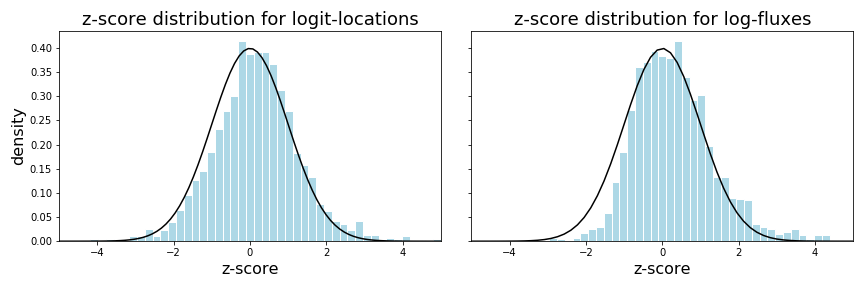
\includegraphics[width=0.99\textwidth]{figures/m2_results/zscore_calibration.png}
    \vspace{-0.5cm}
    \caption{The empirical distribution of z-scores for logit-locations (left) and log-fluxes (right) under the StarNet-WS variational posterior.
}
    \label{fig:z-score_calibration}
\end{figure}

\subsubsection{Runtime}
\label{sec:runtime}
We ran ran SGD to minimize the expected forward KL
for 400 epochs; at each epoch, 200 images were sampled from the generative model.
Optimization was done with Adam~\citep{kingma2014adam}.
On a single NVIDIA GeForce RTX 2080 Ti GPU,
this fitting proceudre took about 50 minutes.

After fitting the model and variational posterior,
calculating the approximate posterior
(that is, producing the distributional parameters of the variational approximation) for the $100 \times 100$ pixel image of M2 took $30$ milliseconds.
By comparison, the reported runtime of PCAT, which uses MCMC, is 30 minutes on the same $100 \times 100$ pixel image~\citep{Feder_2019}.
After the initial fit, StarNet provided nearly a $10^5$-fold speed increase.

The speed at inference time (which excludes training time) gives StarNet the scaling characteristics necessary for processing large astronomical surveys.
A single SDSS image is $1489 \times 2048$ pixels.
Based on the reported 30-minute runtime of PCAT for a $100\times100$ pixel subimage, we project that
the runtime to process the full image would be $30\text{ min} \times 14 \times 20 = 8400$ minutes, or almost six days.
The SDSS survey consists of nearly one million images. Scaling PCAT to the entire SDSS survey would be infeasible.
The upcoming LSST survey will be 300 times larger than SDSS.

In contrast, StarNet only incurs a one-time fitting cost.
After this initial fit,
producing a catalog with the full $1489 \times 2048$ pixel image requires
$30\text{ msec} \times 14 \times 20 = 8.4$ seconds. In practice,
inference can be made even faster by batching the image tiles to run in parallel on a GPU.

In the next subsection, we demonstrate the scaling characteristics on a frame from
the DECAPS survey. 

% Figure~\ref{fig:cmd_m2} displays the estimated color-magnitude diagrams. While the Hubble F606W-band corresponds roughly to the SDSS $r$-band, there is no such correspondence for the SDSS $i$-band. Thus, using the Hubble locations, we estimated the $i$-band fluxes using maximum likelihood: letting $x^{(i)}$ be the SDSS image in the $i$-band, $N_H$ the number of stars in the Hubble catalog and $\ell_H$ their locations, solve
% \begin{align}
%   f^{(i)}_H = \argmax_{f\in\mathbb{R}^{N_H}} \log p(x^{(i)} | N_H, \ell_H, f)
%   \label{eq:optim_iband_flux},
% \end{align}
% where the log likelihood is given by the generative model from Section~\ref{sec:gen_model}.
% The estimated $i$-band fluxes and the reported Hubble F606W-band fluxes $f_H^{(r)}$ define the ``true" colors, $2.5\log(f_H^{(i)}/f_H^{(r)})$.
% In the color magnitude diagram, DAOPHOT did not capture the full spectrum of colors; of all three methods, PCAT best captured the color spectrum. All three methods however, were able to capture the arm thing (TODO there is a name for this ... main sequence turnoff?) that branches off at low magnitudes.

% \begin{figure}[ht]
%     \centering
%     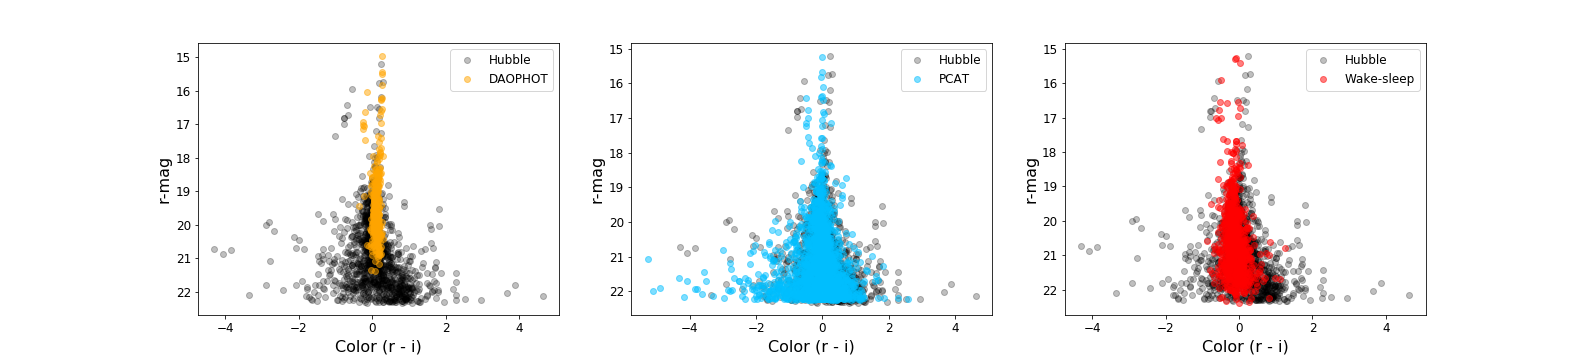
\includegraphics[width=0.99\textwidth]{figures/cmd.png}
%     \caption{Color magnitude diagrams on M2. }
%     \label{fig:cmd_m2}
% \end{figure}



% Figure~\ref{fig:loglik_table} displays the log-likelihood under the default SDSS estimates of the PSF and background compared with the estimates found using wake-sleep.
% The wake-sleep estimates improved the log-likelihood.
% We also compared against the ``Hubble estimate" of the background and PSF, obtained by minimizing $- \log p_\phi(x | N_{H}, \ell_{H}, f_{H})$ for $\phi$ directly.

% The results suggest that the primary source of model misfit is the background. A significant increase in log-likelihood occurred by switching from the SDSS background to the Hubble-estimated background.
% But even using the Hubble-estimated background, switching from the SDSS PSF to our wake-sleep PSF improves the log-likelihood.

% \begin{figure}[ht]
%     \centering
%     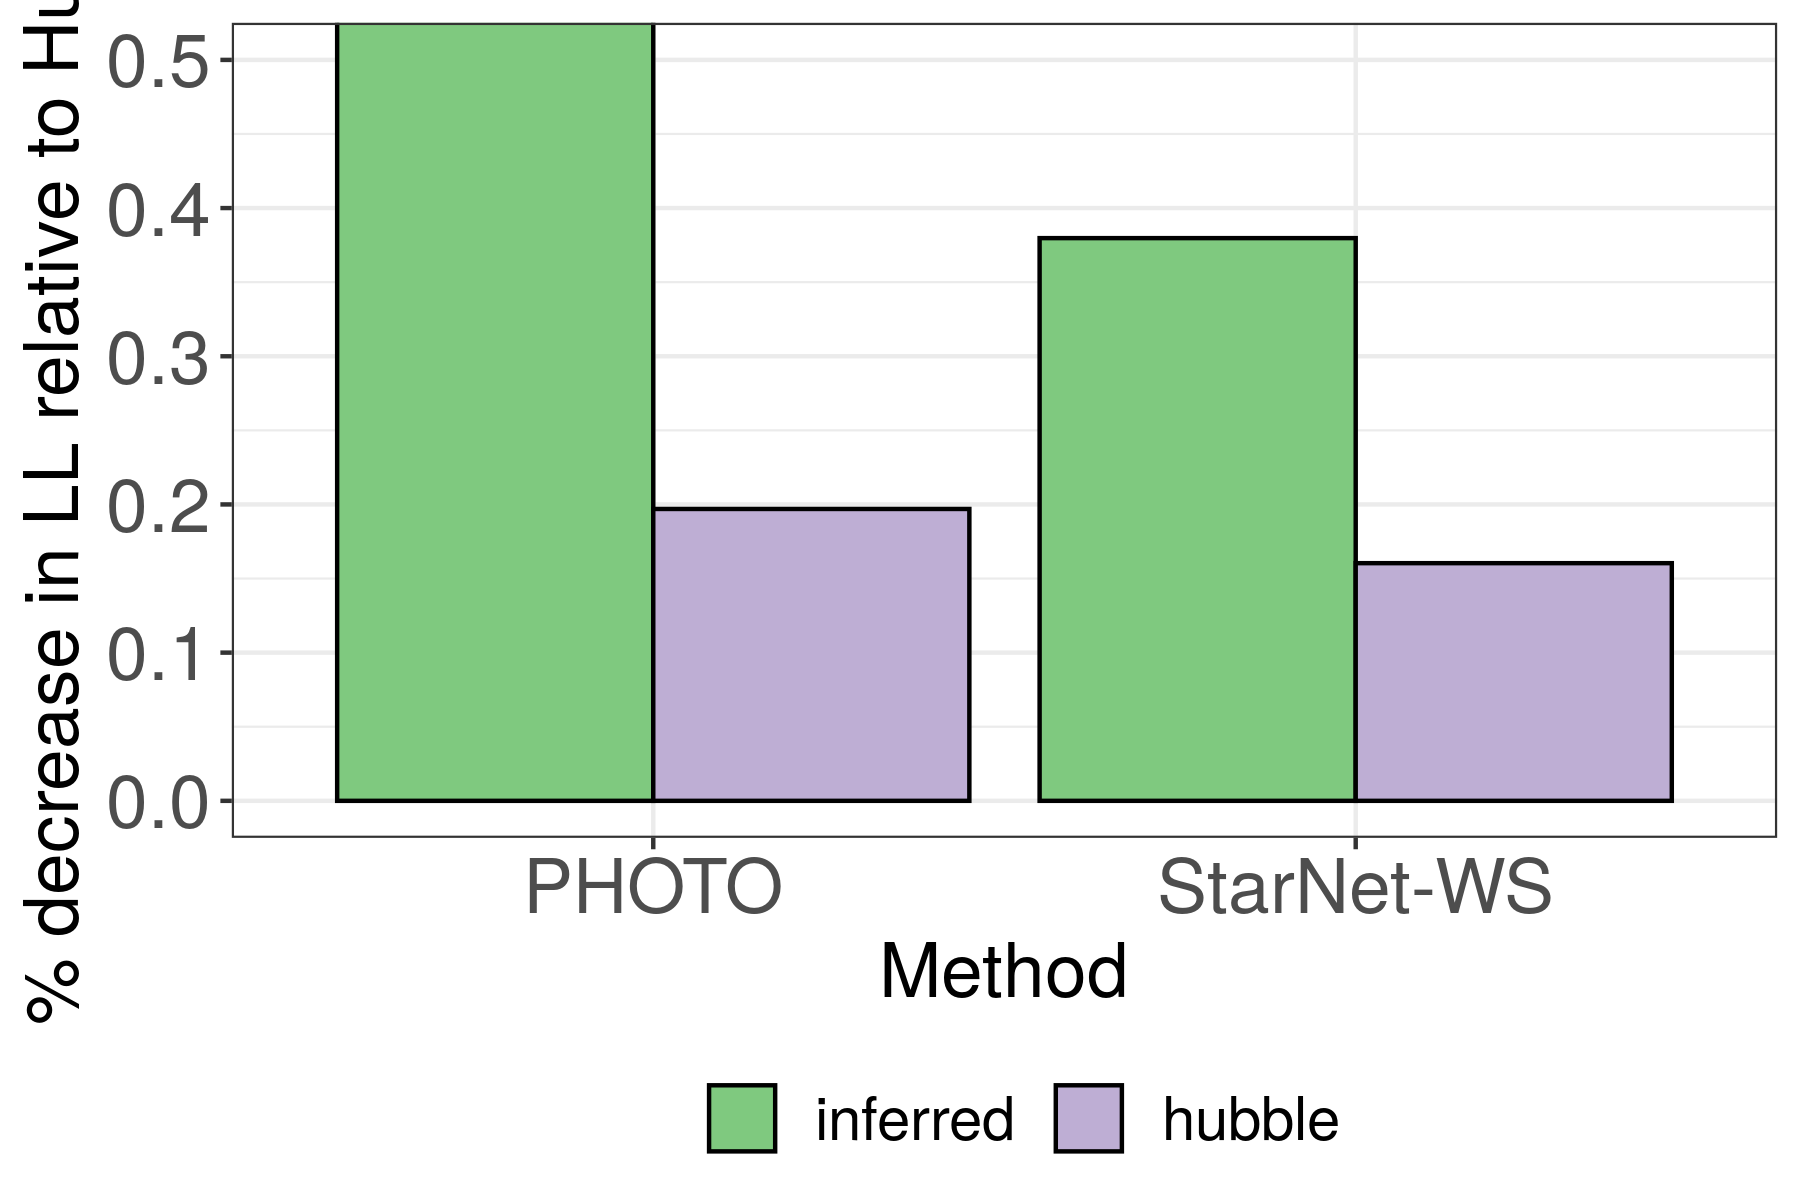
\includegraphics[width=0.6\textwidth]{figures/loglik_table.png}
%     \caption{Percent decrease in log-likelihood relative to the Hubble estimate of the PSF and background.
%     For each method, we evaluate the log-likelihood where the both PSF
%     and background are estimated (green);
%     we also show results where only the PSF is estimated (purple).
%     }
%     \label{fig:loglik_table}
% \end{figure}

% \input{tables/chi_sq_stats.txt}
% \caption{
% Negative log-likelihood for SDSS, wake-sleep, and Hubble estimated model parameters. In the right column, we fix the background to the Hubble estimate, and examine negative log-likelihood as the PSF varies.}

% The StarNet-based PSF did not differ from the SDSS PSF significantly. The greatest change was in the $r$-band PSF, where the SDSS PSF was most different from the Hubble-estimated PSF.

% \begin{figure}[ht]
%     \centering
%     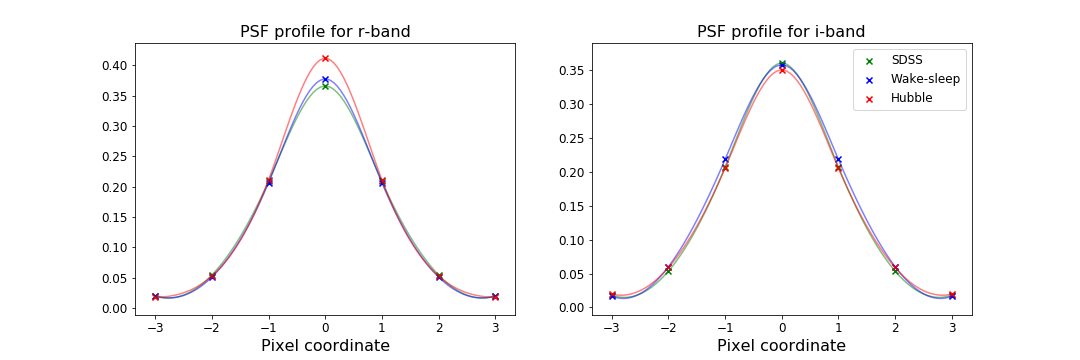
\includegraphics[width=0.99\textwidth]{figures/psf_profiles.png}
%     \caption{Estimated versus true PSF profiles on M2. The Hubble PSF was
%     obtained by optimizing the likelihood conditioned on locations and fluxes
%     from the Hubble catalog. TODO: this image is not that informative, I think I'll remove this. }
%     \label{fig:psf_profiles}
% \end{figure}


% \multicolumn{1}{p{5cm}}{\raggedleft Neg. loglik \\ (with Hubble back.)}
% \caption{
% Chi-squared statistics for SDSS, wake-sleep, and Hubble estimated model parameters.
% The chi-squared statistic is defined as
% $\sum_{bij}\frac{([\text{obs.image}]_{bij} - [\text{recon.image}]_{bij})^2}{[\text{recon.image}]_{bij}}$.
% In the middle column, ``model parameters" refer to both background and PSF.
% In the right column, we fix the background to the Hubble estimate, and examine
% chi-squared statistics as the PSF varies.}


\section{Conclusion}
\label{sec:discussion}
StarNet employs variational inference and outperforms both an MCMC-based probabilistic cataloger and a non-model-based approach in terms of accuracy and runtime. 
Under the framework of probabilistic modeling, 
StarNet produces catalogs in which uncertainties are captured by a Bayesian posterior over the set of all catalogs.
Importantly, unlike MCMC, StarNet also has the capacity to scale probabilistic cataloging to process large astronomical surveys. 

The quality of StarNet detections are the result of optimizing the forward KL, a different objective than the one traditionally used in variational inference. 
Optimizing the forward KL allows the variational posterior to be fit on large amounts of {\itshape complete} data -- the image along with its latent catalog -- generated from the statistical model. 
While labeled data from simulators has been used in other astronomy applications to train deep neural networks (see for example~\cite{Lanusse_2017_cmudeeplens, huang2019finding}), StarNet is the first training procedure to employ simulated data in a statistical framework: the neural network specifies an approximate Bayesian posterior. 

% Our method instead produces an approximate Bayesian posterior using amortized variational inference, which has potential to scale Bayesian inference to large astronomical surveys.
% After a one time cost of training, the network efficiently returns approximate posteriors for batches of images.
% The neural network is trained using the wake-sleep algorithm which optimizes an objective different than the ELBO used in traditional variational inference. 
% In this problem of localizing stars, 
% the ELBO suffers from shallow optimum. 
% The wake-sleep algorithm produced approximate posteriors that were more reliably concentrated around the true catalogs. 
% \jeff{This paper reads a lot like a narrative still. The term ``we'' shows up several hundred times, often unnecessarily, for example. (Perhaps one third of these occurrences could be safely eliminated by reworking sentences.) It's preferable to focus the reader on the model/results rather than on our experiences.
% }
% \jeff{Wake-sleep didn't really avoid the minima---it optimized a different objective entirely.}

This variational approach, unlike previous MCMC approaches, enables StarNet to estimate model parameters such as the PSF and sky background.
While the current work focuses on PSF models, our methodology can be extended to more general sources such as galaxies. 
Unsurprisingly, the current performance of StarNet is sub-optimal for cataloging regions of the sky that contain both stars and galaxies, due to model misfit (Appendix~\ref{sec:results_sparse_field}).  

One promising direction is using a neural network for the generative model and fitting a deep generative model for galaxies~\cite{Arcelin_2020, lanusse2020deep, Reiman_2019_gans_deblend, Regier2015ADG}. 
Here, a neural network encodes a conditional likelihood of galaxy images given a low-dimensional galaxy representation. 
Using a neural network to encode a likelihood extends the flexibility of galaxy models beyond the simple models used here. 


% Going even further, models for artifacts such as cosmic rays and bleed trails~\cite{Desai_2016} could be estimated in this framework.
% \jeff{Readers likely won't know what cosmic rays and bleed trails are. Maybe cite something here that explains them, for the curious reader.}
% These artifacts produce artificial bright spots in an image which do not correspond to celestial objects.
% Currently, pixels corresponding to these objects need to be masked by a preprocessing routine before a catalog can be produced. 
% However, including these artifacts in a statistical model allows for the quantification of uncertainties in their detection. 
% Moreover, credible intervals for latent variables of interest can be computed by marginalizing out the uncertainties in artifact detection. 
% In this way, the uncertainties in artifact detection can be propagated to uncertainties for variables of interest. 

% Our ultimate goal is to provide a pipeline from raw images to catalogs to downstream analyses, where errors are appropriately quantified in each step. 

The statistical framework in this research lays the foundation for building flexible models to incorporate the cataloging of all celestial objects. 
Future astronomical surveys will only expand in terms of the volume of data they are able to amass. 
As telescopes peer deeper into space, fields will reveal more sources and images will become more crowded. 
The uncertainties in crowded fields necessitate a probabilistic approach. 
Our method holds the promise of providing  a scalable inference tool that can meet the challenges of these future surveys. 


% provides a statistical framework for 


% Our method is scalable, works well on deblending, provides approximate inference in achieving this goal .... TODO. 

\jeff{I think there's a bibtex command like ``max\_names'' that will insert et al. You might want to cap the number of names at 6: some of these citations are really long.}
\jeff{A lot of the citations have letters in the wrong case. e.g. ``decam'' instead of ``DECam'', ``lsst'' instead of ``LSST'', ``markov'' instead of ``Markov'', ``Cmu'' instead of ``CMU'', etc.}
\jeff{Also some first names are spelled out in full while others are initials.}

\bibliographystyle{unsrt}
\bibliography{bibliography}

\appendix
\section{Reparameterized and REINFORCE gradients}
\label{sec:reparam_details}
The ELBO objective~\eqref{eq:elbo} is of the form
\begin{align}
    \mathcal{L}(\eta) = \Expect_{q_\eta(z)}[f_\eta(z)].
    \label{eq:gen_elbo}
\end{align}
The parameter $\eta$ is to be optimized, and $z$ is the latent variable. The integrating distribution $q$ and the function $f$ depend on $\eta$.

The REINFORCE estimator~\cite{Williams1992reinforce} is a general-purpose unbiased estimate for the gradient of~\eqref{eq:gen_elbo}.
It is given by
\begin{align}
    g_{\textrm{rf}}(z) = \nabla_\eta f_\eta(z) +
            f_\eta(z)  \nabla_\eta \log q_\eta(z)
    \quad \text{for }
    z\sim q_\eta(z).
\end{align}
The REINFORCE estimate is unbiased for the true gradient:
\begin{align}
    \Expect_{q_\eta(z)}[g_{\textrm{rf}}(z)] &=
    \int q_\eta(z) \nabla_\eta f_\eta(z) \; dz+
    \int q_\eta(z) f_\eta(z)  \nabla_\eta \log q_\eta(z)\; dz \\
    &= \int q_\eta(z) \nabla_\eta f_\eta(z) \; dz+
    \int f_\eta(z) \nabla_\eta q_\eta(z)  \; dz \\
    &= \int \nabla_\eta[q_\eta(z) f_\eta(z)] \; dz \\
    &= \nabla_\eta \int q_\eta(z) f_\eta(z) \; dz
    = \nabla_\eta \Expect_{q_\eta(z)}[f_\eta(z)],
\end{align}
assuming that $f$ is well-behaved so that integration and differentiation can be interchanged.

Alternatively, the reparameterized gradient~\cite{rezende2014stochastic, kingma2013autoencoding} can be used when there exists some distribution $F$ not involving $\eta$ and a differentiable mapping $h_\eta$ such that
\begin{align}
    w \sim F \implies h_\eta(w) \sim q_\eta.
\end{align}
For example, if $q_{\eta}(z) = \mathcal{N}(z; 0, \eta)$ that is, a Gaussian with zero mean and variance $\eta$, one possibility is to let $F$ be the standard Gaussian and $h_\eta(w) = w \sqrt{\eta}$.

The gradient of $\mathcal{L}(\eta)$ can be written as
\begin{align}
    \nabla_\eta \Expect_{q_\eta(z)}[f_\eta(z)] &=
        \nabla_\eta \Expect_{w\sim F}[f_\eta(h_\eta(w)] = \Expect_{w\sim F}[\nabla_\eta f_\eta(h_\eta(w)],
\end{align}
again assuming the interchangability of integrals and derivatives.
Unbiased gradients are computed as
\begin{align}
    g_{\textrm{rp}}
    = \nabla_\eta f_\eta(h_\eta(w))
    = \nabla_z f_\eta(z)\Big|_{z = h_\eta(w)}
    \nabla_\eta h_\eta(w) \quad \text{for } w\sim F.
\end{align}

The reparameterized gradient includes gradient information $\nabla_z f_\eta(z)$ while the REINFORCE gradient does not. Taking into account the structure of $f$ through its gradient lowers the variance of reparameterized gradient in comparison to the REINFORCE gradient.
However, if $z$ contains discrete components, there cannot be a differentiable mapping $h_\eta$, and the reparameterization trick will not apply.

\subsection{Gradients for our ELBO vs sleep experiment}
In Section~\ref{sec:elbo_sleep_compare}, we used a combination of reparameterized and REINFORCE gradients.
Let $N$ be the discrete component of $z$ (the number of stars) and $y$ be the continuous components (the locations and fluxes).
Our variational distribution factorizes, so we write the expectation as
\begin{align}
 \mathcal{L}(\eta) = \Expect_{q_\eta(N)}\Expect_{q_\eta(y)}[f_\eta(N, y)].
 \label{eq:elbo_factorized}
\end{align}
We use the REINFORCE estimator for the outer expectation and the reparameterization trick for the inner expectation. We first apply the REINFORCE to the outer expectation:
\begin{align}
    \nabla_\eta  \Expect_{q_\eta(N)}&\Expect_{q_\eta(y)}\Big[f_\eta(N, y)\Big] \\
    &=  \Expect_{q_\eta(N)}\Big[ \nabla_\eta \log q_\eta(N) \Expect_{q_\eta(y)}[f_\eta(N, y)] +
    \nabla_\eta \Expect_{q_\eta(y)}[f_\eta(N, y)] \Big]\\
    &\approx \nabla_\eta \log q_\eta(N) \Expect_{q_\eta(y)}[f_\eta(N, y)] +
    \nabla_\eta \Expect_{q_\eta(y)}[f_\eta(N, y)] \quad \text{for } N \sim q_\eta(N).
    \label{eq:reinforce_partial}
\end{align}
Then we use the reparameterization trick for $y$, so
\begin{align}
    \Expect_{q_\eta(y)}[f_\eta(N, y)] &\approx f_\eta(N, h_\eta(w))\\
    \nabla_\eta \Expect_{q_\eta(y)}[f_\eta(N, y)] &\approx  \nabla_y f_\eta(N, y)\Big|_{y = h_\eta(w)}
    \nabla_\eta h_\eta(w)
    \label{eq:reparam_partial}
\end{align}
for $w \sim F$, where $h_\eta$ and $F$ are chosen appropriately. Combining~\eqref{eq:reinforce_partial} and~\eqref{eq:reparam_partial}, our gradient estimator is
\begin{align}
    g(z) = \nabla_\eta \log q_\eta(N)
    f_\eta(N, h_\eta(w)) +
    \nabla_y f_\eta(N, y)\Big|_{y = h_\eta(w)}
    \nabla_\eta h_\eta(w)
    \label{eq:appendix_reinforce}
\end{align}
Equation~\ref{eq:appendix_reinforce} is what our main text called the ``REINFORCE gradient."
These gradients produced the optimization path in Figure~\ref{fig:optim_path}(a).

The ``reparameterized" gradient in Section~\ref{sec:elbo_sleep_compare} required integrating out $N$.
Here, we wrote the outer expectation in~\eqref{eq:elbo_factorized} as a summation of $N_{max}$ terms:
\begin{align}
\mathcal{L}(\eta) = \sum_{n=1}^{N_{max}}\Expect_{q_\eta(y)}[f_\eta(n, y)].
\end{align}
Then, the reparameterization trick was applied to each term of the summation.
Stochastic gradients were computed as,
\begin{align}
g(z) = \sum_{n=1}^{N_{max}}\nabla_y f_\eta(n, y)\Big|_{y = h_\eta(w)}
\nabla_\eta h_\eta(w) \quad \text{for } w\sim F.
\end{align}
Gradients of this form produced the optimization path in Figure~\ref{fig:optim_path}(b).


% for $N\sim q_\eta(N)$ and $w\sim F$. Because the variational distribution on locations and fluxes are transformation of Gaussians (recall locations are logit-normal and fluxes log-normal), we take $F$ to be the standard Gaussian, while $h(\cdot ; \eta)$ shifts and scales the standard Gaussian according the the parameters returned by the neural network and applies the appropriate transformation.


\section{Results on Stripe-82}
\label{sec:results_sparse_field}
As discussed in Section~\ref{sec:runtime}, StarNet has potential to scale inference to large astronomical surveys. 
The $100\times100$ image of M2 was chosen as a test bed because a ground truth catalog
could be obtained from Hubble images for validation. 
Moreover, the our point source model is fairly realistic on M2: 
all sources are stars, and there are no galaxies in this region. 
However, most regions of the sky are much less crowded than M2.

SDSS run 94, camcol 1, field  12 is a sparse field more typical of SDSS images. 
After ten minutes of sleep training, StarNet produced a catalog on the full $1489\times 2048$ image in $\approx2$ seconds. For comparison, the projected runtime of PCAT is six days.  

This image is contained in Stripe 82, a region of the sky repeatedly imaged by SDSS. Averaging images from different runs boosts the signal to noise ratio and this {\itshape co-added} image can be analyzed to obtain a ground truth. 

However, this region of the sky also contains galaxies, which are 
not well-modelled by a PSF. A future paper will extend our generative model to include galaxies. For this experiment, only the sleep phase was employed; 
otherwise the model will try to use the PSF to explain both stars and galaxies in the wake-phase. 

Since this region of the sky is more sparse, we tile the image into $50\times 50$ tiles; $N_{max}$ on the tiles is three. 

A $500\times 500$ subimage with the StarNet catalog is shown in 
Figure~\ref{fig:sparse_field_detect}.
Figure~\ref{fig:sparse_field_tpr} reports the TPR, using the coadded catalog as ground truth. 
(We have false defections, namely galaxies, and thus 
do not report the PPV).
The StarNet TPR is comparable with the TPR of the PHOTO catalog. 
Currently, most of the missed detections occur when a large galaxy within a tile causes all $N_{max}$ detections to be placed around the galaxy -- the remaining stars in the image go undetected. 


\begin{figure}
    \centering
    \begin{subfigure}{0.45\textwidth}
        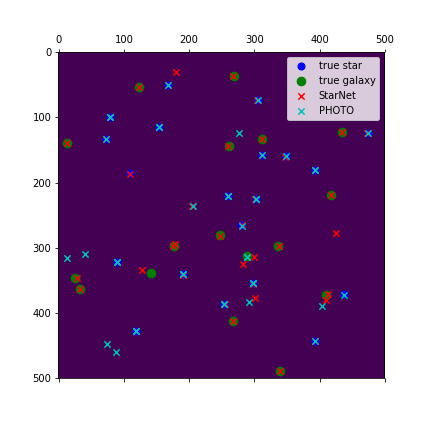
\includegraphics[width=\textwidth]{figures/sparse_field_detections.png}
        \subcaption{}
        \label{fig:sparse_field_detect}
    \end{subfigure}
    \begin{subfigure}{0.54\textwidth}
        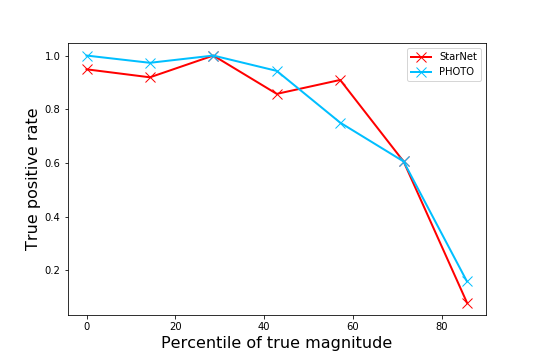
\includegraphics[width=\textwidth]{figures/sparse_field_tpr.png}
        \subcaption{}
        \label{fig:sparse_field_tpr}
    \end{subfigure}
    \caption{(a) a $500\times 500$ sparse field, with true stars in 
    blue, and true galaxies in green. Estimated stars are shown in red x's. 
    (b) the true positive rate as a function of true magnitude. }
    \label{fig:sparse_field}
\end{figure}


\section{Sensitivity to prior parameters}
\label{sec:prior_sensitivity}
We examine the sensitivity of StarNet to prior parameters $\mu$ and $\alpha$ on the image M2. 
Recall $\mu$ is the prior mean number of stars per pixel~\eqref{eq:n_prior};
$\alpha$ is the power law slope on the $r$-band fluxes~\eqref{eq:flux_prior}. 
In the results of Section~\ref{sec:results_on_m2}, $\mu=0.15$ and  $\alpha = 0.5$. 

The model appears reasonably robust. 
As expected, as $\mu$ increases the TPR increases while the PPV decreases  -- the prior encourages more detections (Figure~\ref{fig:mu_sensitivity}). 

\begin{figure}[ht]
\begin{subfigure}{\textwidth}
\centering
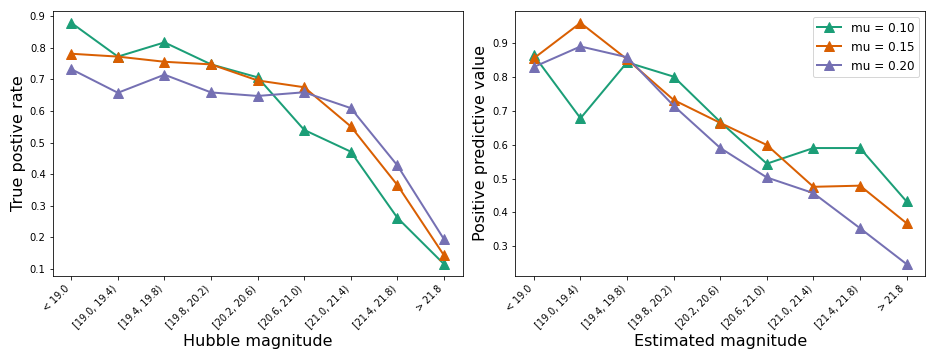
\includegraphics[width = \textwidth]{figures/prior_sensitivity/prior_mu_sensitivty.png}
\end{subfigure}
\begin{subfigure}{\textwidth}
\begin{center}
\begin{tabular}{rrr}
\toprule
     mu &   TPR &   PPV \\
\midrule
 0.10 &  0.46 &  0.66 \\
 0.15 &  0.51 &  0.60 \\
 0.20 &  0.51 &  0.49 \\
\bottomrule
\end{tabular}
\par\vspace{0pt}
\end{center}
\end{subfigure}\hfill
\caption{Sensitivity of performance metrics to Poisson mean parameter on number of stars. }
\label{fig:mu_sensitivity}
\end{figure}

As $\alpha$ increases, StarNet estimates more dim sources: the prior distribution on fluxes places more mass near $f_{min}$ (Figure~\ref{fig:flux_priors}). 

\begin{figure}[!h]
    \centering
    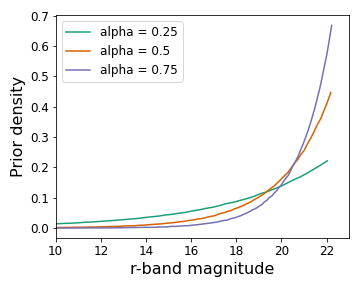
\includegraphics[width = 0.6\textwidth]{figures/prior_sensitivity/prior_fluxes.png}
    \caption{The prior density of $r$-band magnitude for various power law slopes $\alpha$}
    \label{fig:flux_priors}
\end{figure}

While the TPR increases across $\alpha$ values, the PPV suffers at $\alpha = 0.75$ (Figure~\ref{fig:alpha_sensitivity}).
At $\alpha = 0.75$, we see that the TPR improves at dimmer sources at the expense of brighter sources, suggesting that the brigher sources become over-split. 
The stronger prior on dimmer stars also manifests in the flux distribution of the resulting StarNet catalog (Figure~\ref{fig:cdf_sensitivity}). 

\begin{figure}[ht]
\begin{subfigure}{\textwidth}
\centering
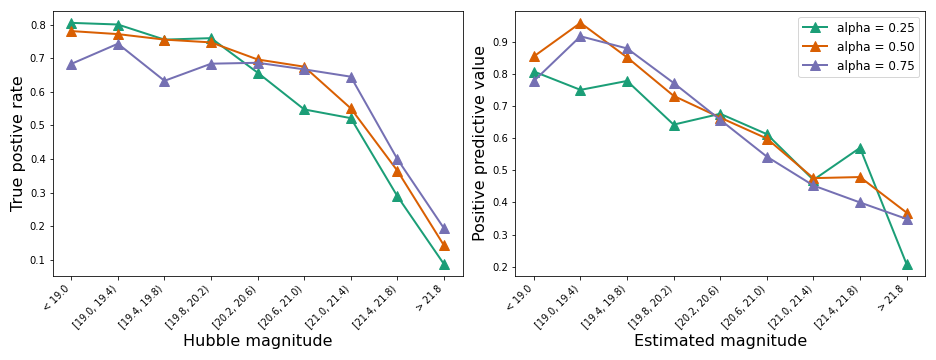
\includegraphics[width = \textwidth]{figures/prior_sensitivity/prior_alpha_sensitivity.png}
\end{subfigure}
\begin{subfigure}{\textwidth}
\begin{center}
\begin{tabular}{rrr}
\toprule
 alpha &   TPR &   PPV \\
\midrule
  0.25 &  0.46 &  0.60 \\
  0.50 &  0.51 &  0.60 \\
  0.75 &  0.52 &  0.54 \\
\bottomrule
\end{tabular}
\par\vspace{0pt}
\end{center}
\end{subfigure}\hfill
\caption{Sensitivity of performance metrics to flux prior parameter $\alpha$. }
\label{fig:alpha_sensitivity}
\end{figure}

\begin{figure}
    \centering
    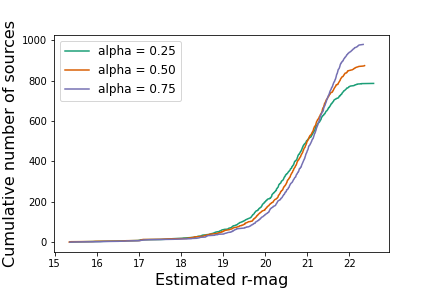
\includegraphics[width = 0.6\textwidth]{figures/prior_sensitivity/sensitivity_cdf_fluxes.png}
    \caption{Sensitivity of estimated flux distribution to flux prior parameter $\alpha$.}
    \label{fig:cdf_sensitivity}
\end{figure}

% probably won't include these sections anymore
% \section{Results on a test M2 image}
% In this section, we evaluate our approximate posterior on another subimage of M2. Figure~\ref{fig:marked_m2} is an image of M2. In red is the subimage considered in the body of the paper. 
We ran the wake-sleep algorithm on the red region, and here, we examine the results on the blue image. 


\begin{figure}
    \centering
    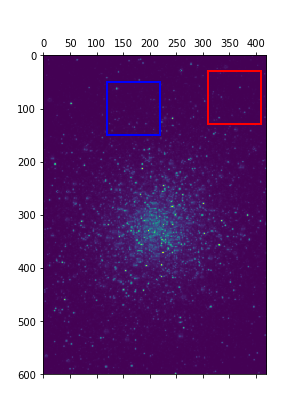
\includegraphics{figures/sdss_m2_image2_marked.png}
    \caption{An image of M2. We trained the wake-sleep algorithm on the red subregion, and evaluated our variational posterior in the blue region. }
    \label{fig:marked_m2}
\end{figure}

\begin{figure}[ht]
\begin{subfigure}{\textwidth}
\centering
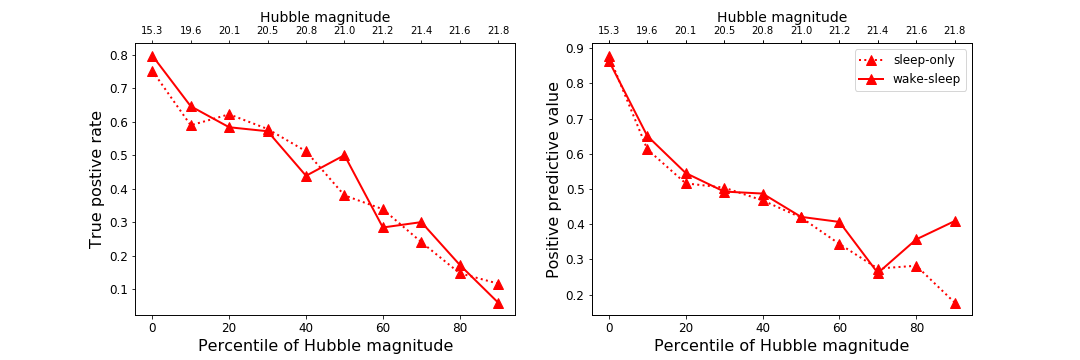
\includegraphics[width = \textwidth]{figures/summary_statistics_m2_alt.png}
\end{subfigure}
\begin{subfigure}{\textwidth}
\begin{center}
\begin{tabular}{lrrr}
\toprule
 &   TPR &   PPV &  F1 score  \\
\midrule
 Sleep-only &  0.51 &  0.47 &      0.49 \\
 Wake-sleep &  0.49 &  0.64 &      0.56  \\
Sleep-only (test) &  0.43 &  0.45 & 0.44 \\
 Wake-sleep (test) &  0.40 &  0.53 &      0.45  \\
\bottomrule
\end{tabular}
\par\vspace{0pt}
\end{center}
\end{subfigure}\hfill
\caption{Results on the test region of M2. }
\end{figure}


% \section{Comparison with importance sampling}
\label{sec:compare_w_is}

TODO: here, I look at results on a small $8 \times 8$ image in one band. I see how well we are able to deblend the image. 

Preliminary results are in Figure~\ref{fig:deblending_test}. 

I display the log-odds, $\log q(N = 2)  - \log q(N = 1)$, under our sleep-trained variational posterior. 

I compare against the true posterior, computed by gridding the sample space: we took a grid of $100\times 100$ locations and $100$ fluxes (for two stars, this had to be squared, for a total of $100^6$ samples ... it took awhile). 

Interestingly, the true posterior is biased towards two stars, even when the two stars are perfectly overlapping.

This actually makes sense. When two stars are perfectly overlapping (source separation = 0), the likelihood conditional on one bright star vs. the likelihood conditional on two stars each with half the brightness of the one star will be exactly the same. The prior (Poisson mean = 1) slightly encourages one star over two, but the flux distribution (which encourages dimmer stars) implicitly encourages two stars. In this example, these two prior terms seem to balance out. We see that when the separation is zero, the log-odds is about zero. 

Unfortunately, our variational posterior doesn't have the same behavior. The neural net just doesn't seem good enough to detect that there should be two stars? Also, the network seems very confident -- the log odds jump quickly from -5 (super confident of 1 star) to to 0.4 to 1 (super confident of two stars). 

\begin{figure}[!h]
    \centering
    \begin{subfigure}[t]{\textwidth}
    \centering
    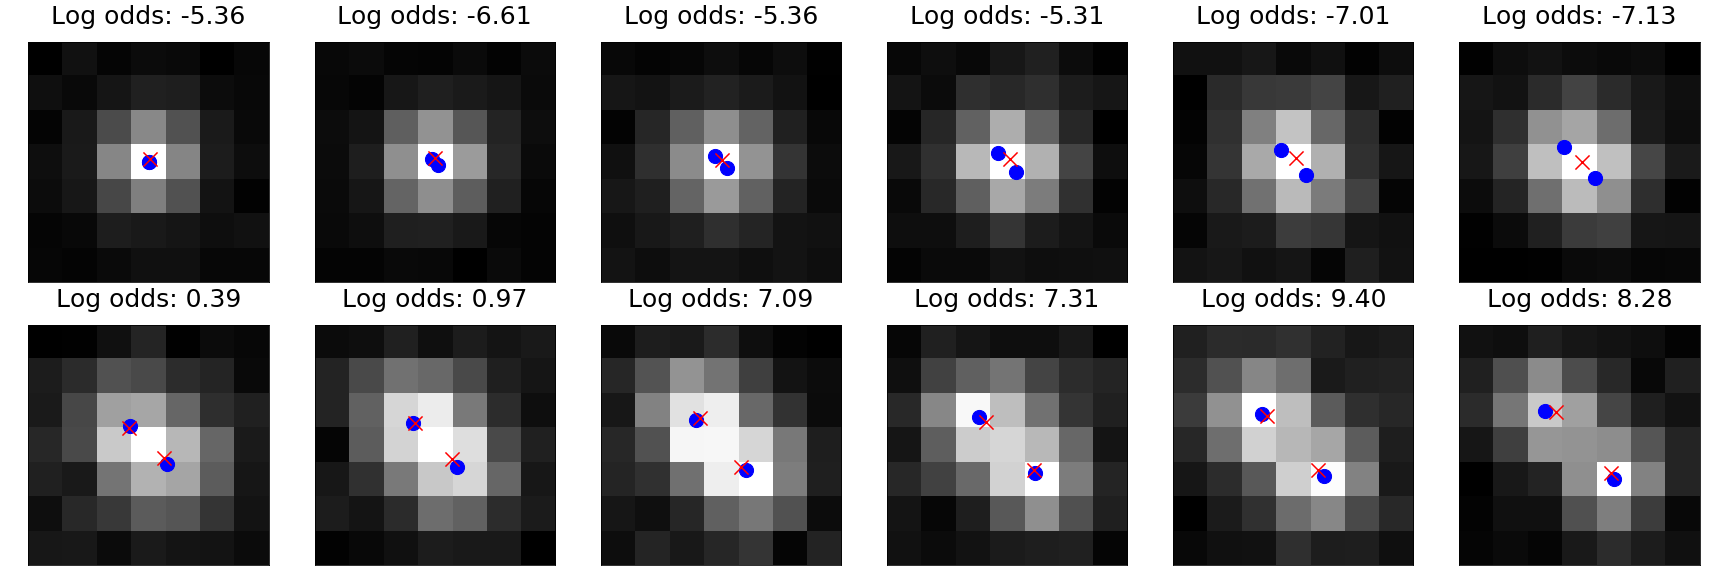
\includegraphics[width=\textwidth]{figures/deblending_ex.png}
    \end{subfigure}
    \begin{subfigure}[t]{\textwidth}
    \centering
    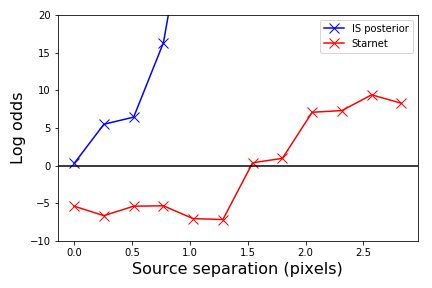
\includegraphics[width=0.5\textwidth]{figures/deblending_is_compare.png}
    \end{subfigure}
    \vspace{-3em}
    \caption{(Top) Detections as source separation increases. Red are MAP detections, blue are true locations. Log odds displayed are probability of two stars over probability of one star (Bottom) Comparison of log odds from the variational posterior and from the true posterior; the latter is computed by importance sampling. }
    \label{fig:deblending_test}
\end{figure}


In the final draft, I would also like have a more wide-ranging deblending test, similar to Figure 5 in~\cite{Feder_2019}, where we look at how well we deblend stars as fluxes and colors vary. 


\end{document}
